\section{Subgroups}

\subsection{Definitions and Examples}

\begin{problems}
    \item In each of (a)–(e) prove that the specified subset is a subgroup of the given group:
    \begin{problems}
        \item the set of complex numbers of the form $a + ai$, $a \in \mathbb{R}$ (under addition)
        \item the set of complex numbers of absolute value $1$, i.e., the unit circle in the complex plane (under multiplication)
        \item for fixed $n \in \mathbb{Z}^+$ the set of rational numbers whose denominators divide $n$ (under addition)
        \item for fixed $n \in \mathbb{Z}^+$ the set of rational numbers whose denominators are relatively prime to $n$ (under addition)
        \item the set of nonzero real numbers whose square is a rational number (under multiplication)
    \end{problems}
    \begin{sol}
        Let $G$ be the group in question and let $H$ be the set that we are trying to prove is a subgroup of $G$.
        \begin{problems}
            \item Clearly $0 = 0 + 0i \in H$ so that $H$ is nonempty. Suppose $a + ai, b + bi \in H$. Then $a - b \in \r$ so that $(a + ai) - (b + bi) = (a - b) + (a - b)i \in H$ so that $H \leq G$.
            \item Since $\abs 1 = 1$, then $1 \in H$ so that it is nonempty. Suppose $z, w \in H$. Note that $\abs{w\inv} = 1$ since $\abs{w\inv} = \abs{\bar w}/\abs {w}^2 = 1/1 = 1$. Then
            \[\abs{zw\inv} = \abs z \abs{w\inv} = (1)(1) = 1\]
            so that $zw\inv \in H$. Then $H \leq G$.
            \item Let $n \in \zp$ be fixed. Since $0 = 0/k$ where $k \mid n$, then $0 \in H$ so that it is nonempty. Suppose $a/b, c/d \in H$, where $(a, b) = (c, d) = 1$, and $br = ds = n$ for $r, s \in \z$. Then
            \[\frac ab - \frac cd = \frac{ar}n - \frac{cs}n = \frac{ar - bs}n\]
            After reduction, the denominator will still be a divisor of $n$, so $a/b - c/d \in H$, and $H \leq G$.
            \item Fix $n \in \zp$, and note that $0= 0/1 \in H$ so that $H$ is nonempty. Suppose $a/b, c/d \in H$ such that $(b, n) = (d, n) = 1$. For any prime $p$ such that $p \mid n$, then $p \nmid b$ and $p \nmid d$. Then
            \[\frac ab - \frac cd = \frac{ad - bc}{bd}\]
            Consider $x = (bd, n)$. Then $p \nmid x$, for otherwise $p \mid bd$ implying that $p \mid b$ or $p \mid d$. Then $x = 1$, and $a/b - c/d \in H$ so that $H \leq G$.
            \item Since $1 = 1^2 = 1/1 \in H$, then $H$ is nonempty. Suppose $a, b \in H$. Then $a^2, b^2 \in \q$ so that
            \[\left(\frac ab\right)^2 = \frac{a^2}{b^2} \in H\]
            then $a/b \in H$, and $H \leq G$. \qh
        \end{problems}
    \end{sol}
    \item In each of (a)–(e) prove that the specified subset is \emph{not} a subgroup of the given group:
    \begin{problems}
        \item the set of $2$-cycles in $S_n$ for $n \ge 3$
        \item the set of reflections in $D_{2n}$ for $n \ge 3$
        \item for $n$ a composite integer $>1$ and $G$ a group containing an element of order $n$, the set $\{x \in G \mid |x| = n\} \cup \{1\}$
        \item the set of (positive and negative) odd integers in $\mathbb{Z}$ together with $0$
        \item the set of real numbers whose square is a rational number (under addition)
    \end{problems}
    \begin{sol}
        Let $H$ be the set in question and $G$ be the group.
        \begin{problems}
            \item Note that $(1\ 2), (1\ 3) \in H$, but $(1\ 2)(1\ 3) = (1\ 3\ 2) \not\in H$.
            \item $s, sr \in H$, but $s(sr) = r \not\in H$ as $r$ is not a reflection.
            \item Let $p \in \zp$ such that $p \mid n$. Pick $x \in H$ so that $x^{n/p} \in H$. But $|x^{n/p}| < n$, since $(x^{n/p})^p = x^n = 1$, so $H$ is not closed under the operation.
            \item $1 \in H$, but $1 + 1 = 2 \not\in H$.
            \item $\sqrt 2, \sqrt 3 \in H$, but $(\sqrt 2 + \sqrt3)^2 = 2 + 2\sqrt6 + 3 \not\in H$, so $\sqrt 2 + \sqrt 3 \not\in H$. \qh
        \end{problems}
    \end{sol}
    \item Show that the following subsets of the dihedral group $D_8$ are actually subgroups:
    \begin{problems}
        \item $\{1, r^2, s, sr^2\}$
        \item $\{1, r^2, sr, sr^3\}$
    \end{problems}
    \begin{solalph}
        \item 
        \[
        \begin{array}{c|cccc}
            \circ & 1 & r^2 & s & sr^2 \\
            \hline
            1 & 1 & r^2 & s & sr^2 \\
            r^2 & r^2 & 1 & sr^2 & s \\
            s & s & sr^2 & 1 & r^2 \\
            sr^2 & sr^2 & s & r^2 & 1
        \end{array}
        \]
        \item 
        \[
        \begin{array}{c|cccc}
            \circ & 1 & r^2 & sr & sr^3 \\
            \hline
            1 & 1 & r^2 & sr & sr^3 \\
            r^2 & r^2 & 1 & sr^3 & sr \\
            sr & sr & sr^3 & 1 & r^2 \\
            sr^3 & sr^3 & sr & r^2 & 1
        \end{array}
        \]
        Both tables show closure, since no product is an element outside of the subset.
    \end{solalph}
    \item Give an explicit example of a group $G$ and an infinite subset $H$ of $G$ that is closed under the group operation but is not a subgroup of $G$.
    \begin{sol}
        Consider $\zp$ and $\z$ under addition. Then $|\zp| = \infty$ and $m + n \in \zp$ for any $m, n \in \zp$, but $m - n \not\in \zp$ when $m < n$. Then $\zp$ is not a subgroup of $\z$.
    \end{sol}
    \item Prove that $G$ cannot have a subgroup $H$ with $|H| = n - 1$, where $n = |G| > 2$.
    \begin{sol}
        Suppose that there did exist $H$ such that $|H| = n - 1$. By Lagrange's Theorem, then $n - 1 \mid n$. Then there exists $k$ such that $k(n - 1) = kn - k = n$, or that $n = k/(k - 1)$. Since $n > 2$, we may safely assume that $k > 2$. Since $n \not\in \zp$ for any $k > 2$, this contradicts Lagrange's Theorem.
    \end{sol}
    \item Let $G$ be an abelian group. Prove that $\{ g \in G \mid |g| < \infty \}$ is a subgroup of $G$ (called the torsion subgroup of $G$). Give an explicit example where this set is not a subgroup when $G$ is non-abelian.
    \begin{sol}
        Let $\tor(G)$ denote the torsion subgroup of $G$. Since $\abs 1 = 1$, then $1 \in \tor(G)$. Now suppose $g, h \in \tor(G)$, and put $\abs g = m$ and $\abs h = n$ for finite $m, n$. Then
        \[(gh\inv)^{mn} = g^{mn}(h\inv)^{mn} = (g^m)^n((h\inv)^n)^m = 1^n1^m = 1\]
        so that $gh\inv \in \tor(G)$. Then $\tor(G) \leq G$.
        
        Now suppose $G = \aut(\r)$ and consider $\tor(G) = \{f \in \aut(\r) \mid \abs f < \infty\}$. Then $f(x) = -x$ and $g(x) = 1/x$ are both in $\tor(G)$, since $f^2(x) = g^2(x) = x$, but $f(g(x)) = -1/x \not\in \tor(G)$, since $(f \circ g)^n(x) = (-1)^nx^{(-1)^n} \neq 1$ for any $n \in \z$.
    \end{sol}
    \item Fix some $n \in \mathbb{Z}$ with $n>1$. Find the torsion subgroup (cf. the previous exercise) of $\mathbb{Z} \times (\mathbb{Z}/n\mathbb{Z})$. Show that the set of elements of infinite order together with the identity is \emph{not} a subgroup of this direct product.
    \begin{sol}
        Since every nonidentity element of $\z$ has infinite order, then $\tor(\z \times \intmod) = \{(0, x) \mid x \in \intmod\}$, since every $x \in \intmod$ has finite order as $\intmod$ is finite. Moreover, if we let $H$ be the set of elements of infinite order along with the identity $(0, 0)$, then $(1, 1), (-1, 0) \in H$, but $(1, 1) + (-1,0) = (0, 1) \not\in H$ because it belongs to the torsion subgroup. 
    \end{sol}
    \item Let $H$ and $K$ be subgroups of $G$. Prove that $H \cup K$ is a subgroup if and only if either $H \subseteq K$ or $K \subseteq H$.
    \begin{sol}
        Suppose $H \cup K$ is a subgroup. If $H \subseteq K$, we are done. Now suppose $H \not\subseteq K$. Then there exists $h \in H$ such that $h \not\in K$. Let $k \in K$. Then $hk \in H \cup K$. If $hk \in K$, then $hk(k\inv) = h \in K$, which is a contradiction. Then $hk \in H$. Then $h\inv \in H$ so that $h\inv(hk) = k \in H$ so that $K \subseteq H$.
        
        If $H \subseteq K$ then $H \cup K = K$. If $K \subseteq H$, then $H \cup K = H$, both of which are subgroups of $G$. The result follows.
    \end{sol}
    \item Let $G = \gl_n(F)$, where $F$ is any field. Define
    \[\speclin_n(F) = \{ A \in \gl_n(F) \mid \det(A) = 1 \}\]
    (called the special linear group). Prove that $\speclin_n(F) \le \gl_n(F)$.
    \begin{sol}
        Since $\det(I_n) = 1$, then $I_n \in \speclin_n(F)$ so that $\speclin_n(F)$ is nonempty. Suppose $A, B \in \speclin_n(F)$. Then
        \[\det(AB\inv) = \det(A)\det(B\inv) = \frac{\det(A)}{\det(B)} = \frac 11 = 1\]
        so that $AB\inv \in \speclin_n(F)$. It follows that $\speclin_n(F) \leq \gl_n(F)$.
    \end{sol}
    \item 
    \begin{problems}
        \label{ex2.1.10}
        \item Prove that if $H$ and $K$ are subgroups of $G$ then so is their intersection $H \cap K$.
        \item Prove that the intersection of an arbitrary nonempty collection of subgroups of $G$ is again a subgroup of $G$ (do not assume the collection is countable).
    \end{problems}
    \begin{solalph}
        \item Put $L = H \cap K$. Since $1 \in H$ and $1 \in K$, then $1 \in L$ so that $L$ is nonempty. Pick $a, b \in L$. Then $a, b \in H$ and $a, b \in K$. Then $ab\inv \in H$ and $ab\inv \in K$ so that $ab\inv \in L$, hence $L \leq G$.
        \item Let $H_i$ be a subgroup of $G$ with $i$ belonging to an indexing set $I$. Let
        \[H = \bigcap_{i \in I}H_i\]
        Since $1 \in H_i$ for all $i$, then $1 \in H$. Suppose $a, b \in H$. Then $a, b \in H_i$ so that $ab\inv \in H_i$ for all $i \in I$. It follows that $ab\inv \in H$, hence $H \leq G$.
    \end{solalph}
    \item Let $A$ and $B$ be groups. Prove that the following sets are subgroups of the direct product $A \times B$:
    \begin{problems}
        \item $\{ (a, 1) \mid a \in A \}$
        \item $\{ (1, b) \mid b \in B \}$
        \item $\{ (a, a) \mid a \in A \}$, where we assume $B = A$ (called the diagonal subgroup)
    \end{problems}
    \begin{sol}
        Let $C$ be the set in each part.
        \begin{problems}
            \item Since $1 \in A$, then $(1, 1) \in C$ so that $C$ is nonempty. Suppose $(a_1, 1), (a_2, 1) \in C$ for $a_1, a_2 \in A$. Then $a_1a_2\inv \in A$. Then
            \[(a_1, 1)(a_2, 1)\inv = (a_1, 1)(a_2\inv, 1) = (a_1a_2\inv, 1) \in C\]
            so that $C \leq A \times B$.
            \item See above proof, but suppose $(1, b_1), (1, b_2) \in C$ for $b_1, b_2 \in B$.
            \item $1 \in A$ so $(1, 1) \in C$, and $C$ is nonempty. For $a_1, a_2 \in A$, then $a_1a_2\inv \in A$ so that
            \[(a_1, a_1)(a_2, a_2)\inv = (a_1a_2\inv, a_1a_2\inv) \in C\]
            so that $C \leq A^2$. \qh
        \end{problems}
    \end{sol}
    \item Let $A$ be an abelian group and fix some $n \in \mathbb{Z}$. Prove that the following sets are subgroups of $A$:
    \begin{problems}
        \item $\{ a^n \mid a \in A \}$
        \item $\{ a \in A \mid a^n = 1 \}$
    \end{problems}
    \begin{sol}
        Let $B$ be the sets in question.
        \begin{problems}
            \item $1^n = 1$, so $1 \in B$. Suppose $a^n, b^n \in B$. Then
            \[(a^n)(b^n)\inv = (a^n)(b\inv)^n = (ab\inv)^n\]
            where the last equality follows, since $A$ is abelian. Then $ab\inv \in B$, hence $B \leq A$.
            \item $1^n = 1$, so $1 \in B$. Suppose $a, b \in B$. Then
            \[(ab\inv)^n = a^n(b^n)\inv = 1(1\inv) = 1\]
            so that $ab\inv \in B$, and $B \leq A$. \qh
        \end{problems}
    \end{sol}
    \item Let $H$ be a subgroup of the additive group of rational numbers with the property that $1/x \in H$ for every nonzero element $x$ of $H$. Prove that $H = 0$ or $\mathbb{Q}$.
    \begin{sol}
        Let $H \leq \q$. Then $0 \in H$. If no other element is in $H$, then $H = 0$ and we are done. Suppose that $H \neq 0$ so that there exists $x = a/b \in H$. Moreover, we may take $x > 0$, because if $x < 0$, take $-x > 0$ instead since $H$ has inverses. Note that $bx = a \in H$ so that $1/a \in H$. Then $a(1/a) = 1 \in H$. Then $\z \subseteq H$, since we may use 1 to build every integer.
        
        Now suppose $r \in \q$, and put $r = p/q$ for $p, q \in \z$. Then $q \in H$ so that $1/q \in H$, hence $p(1/q) = r \in H$. Then $\q \subseteq H$, and $H = \q$.
    \end{sol}
    \item Show that $\{ x \in D_{2n} \mid x^2 = 1 \}$ is \emph{not} a subgroup of $D_{2n}$ (here $n \ge 3$).
    \begin{sol}
        Let $H$ be the set in question. Then $s, sr \in H$, since $|s| = 2$, and $(sr)^2 = s(sr\inv)r = 1$. But $s(sr) = r \not\in H$, because $\abs r \geq 3$.
    \end{sol}
    \item Let $H_1 \subseteq H_2 \subseteq \cdots$ be an ascending chain of subgroups of $G$. Prove that $\bigcup_{i=1}^\infty H_i$ is a subgroup of $G$.
    \begin{sol}
        Let $H = \bigcup_{i = 1}^\infty H_i$. Since $1 \in H_i$ for all $i$, then $1 \in H$ so that $H$ is nonempty. Pick $a, b \in H$. Then $a \in H_i$ and $b \in H_j$ for some $i, j \in \zp$. Then $a, b \in H_k$, where $k = \max(i, j)$. Then $ab\inv \in H_k$ so that $ab\inv \in H$, hence $H \leq G$.
    \end{sol}
    \item Let $n \in \mathbb{Z}^+$ and let $F$ be a field. Prove that the set $\{ (a_{ij}) \in \gl_n(F) \mid a_{ij} = 0 \text{ for all } i > j \}$ is a subgroup of $\gl_n(F)$ (called the group of upper triangular matrices).
    \begin{sol}
        Let $\ut_n(F)$ denote the set of $n \times n$ upper triangular matrices with entries from $F$. Since $I_n$ has all $0$s except the diagonal, then $I_n \in \ut_n(F)$ so that $\ut_n(F)$ is nonempty. Suppose $A, B \in \ut_n(F)$. Since $A, B \in \gl_n(F)$, then $\det(A)$ and $\det(B)$ are nonzero. Putting $AB = C = (c_{ij})$ it follows that $\det(C)$ is also nonzero. Note that
        \[c_{ij} = \sum_{k = 1}^n a_{ik}b_{kj}\]
        Suppose $i > j$. Then if $i > k$, then $a_{ik} = 0$, and if $k > j$, then $b_{kj} = 0$ so that $c_{ij} = 0$, hence $C \in \ut_n(F)$.
        
        To show that $A\inv \in \ut_n(F)$, put $D \in \ut_n(F)$ such that $AD = DA = I_n$. Proceeding by induction, we show the case for $n = 2$: Consider the matrices
        \[A = 
        \begin{pmatrix}
            a_{11} & a_{12} \\
            0 & a_{22}
        \end{pmatrix}, \quad
        D = 
        \begin{pmatrix}
            d_{11} & d_{12} \\
            d_{21} & d_{22}
        \end{pmatrix}
        \]
        such that $AD = I_2$. While we may solve for each $d_{ij}$ explicitly, since $D \in \gl_2(F)$, it must be that $d_{ii} \neq 0$, and $d_{12} \in F$, so it remains to show that $d_{21} = 0$. To that end, note that $a_{22}d_{21} = 0$. Since $a_{22} \neq 0$ (otherwise $\det(A) = 0$ and $A \not\in \gl_2(F)$), it must be that $d_{21} = 0$, hence $D \in \ut_2(F)$. Suppose now that the inverse $D$ of $A \in \gl_n(F)$ is also upper triangular, and consider $A \in \ut_{n + 1}(F)$ and $D \in \gl_{n + 1}(F)$ such that $AD = DA = I_{n + 1}$. Using block matrices, we may write this as
        \[
        \begin{pmatrix}
            A_0 & \b a_{12} \\
            0 & a_{22}
        \end{pmatrix}
        \begin{pmatrix}
            D_0 & \b d_{12} \\
            \b d_{21}^T & d_{22}
        \end{pmatrix} = 
        \begin{pmatrix}
            D_0 & \b d_{12} \\
            \b d_{21}^T & d_{22}
        \end{pmatrix}
        \begin{pmatrix}
            A_0 & \b a_{12} \\
            0 & a_{22}
        \end{pmatrix} = 
        \begin{pmatrix}
            I_n & \b 0_{n \times 1} \\
            \b 0_{n \times 1}^T & 1
        \end{pmatrix}
        \]
        where $\b a_{12}, \b d_{12}, \b d_{21}^T, \b 0_{n \times 1}^T$ are $n \times 1$ column vectors, and $a_{22}, d_{22} \in F$. We can see that $D_0A_0 = I_n$ so that $D_0 \in \ut_n(F)$ by assumption. Moreover, $a_{22}\b d_{21}^T = \b 0_{n \times 1}^T$. Since $a_{22} \neq 0$ because $A \in \ut_{n + 1}(F)$, then $\b d_{21}^T = \b 0_{n \times 1}^T$. By induction, then $D \in \ut_{n + 1}(F)$, hence the inverse of any upper triangular matrix is also upper triangular.
    \end{sol}
    \item Let $n \in \mathbb{Z}^+$ and let $F$ be a field. Prove that the set $\{ (a_{ij}) \in \gl_n(F) \mid a_{ij} = 0 \text{ for all } i > j,\ \text{and } a_{ii} = 1 \text{ for all } i \}$ is a subgroup of $\gl_n(F)$.
    \begin{sol}
        Let $H$ be the set in question. Since the diagonal of $I_n$ is only 1's, then $I_n \in H$. Suppose $A, B \in H$. By the previous exercise, $A, B \in \ut_n(F)$, so it remains to show that $a_{ii} = b_{ii} = 1$ for all $1 \leq i \leq n$. Then
        \[(AB)_{ii} = \sum_{k = 1}^n a_{ik}b_{ki}\]
        Since $a_{ik} = 0$ for $k < i$ and $b_{ki} = 0$ for $k > i$, then the sum degrades to $a_{ii}b_{ii} = 1$. Then $H$ is closed under multiplication. Moreover, suppose $D \in \ut_n(F)$ such that $DA = I_n$. Then
        \[1 = (DA)_{ii} = d_{ii}a_{ii}\]
        where we use the above to collapse the $ii$-th term of $DA$. Then $d_{ii} = 1$, hence $D \in H$, and $H$ is closed under inverses. Hence, $H \leq \gl_n(F)$.
    \end{sol}
\end{problems}

\newpage

\subsection{Centralizers and Normalizers, Stabilizers and Kernels}

\begin{problems}
    \item Prove that $C_G(A)=\{g\in G\mid g^{-1}ag=a\text{ for all }a\in A\}.$
    \begin{sol}
        $g \in C_G(A)$ if and only if $gag\inv = a$ if and only if $a = g\inv ag$.
    \end{sol}
    \item Prove that $C_G(Z(G))=G$ and deduce that $N_G(Z(G))=G.$
    \begin{sol}
        Recall that $C_G(Z(G)) = \{g \in G \mid gag\inv = a \text{ for all } a \in Z(G)\}$. Clearly $C_G(Z(G)) \subseteq G$. Now suppose $g \in G$ and pick $z \in Z(G)$. Then $gz = zg$, or $gzg\inv = z$. Then $g \in C_G(Z(G))$, hence $G \subseteq C_G(Z(G))$. It follows that $C_G(Z(G)) = G$. Moreover, because $G = C_G(Z(G)) \leq N_G(Z(G))$ and $N_G(Z(G)) \leq G$ by definition, then $N_G(Z(G)) = 0$.
    \end{sol}
    \item Prove that if $A$ and $B$ are subsets of $G$ with $A \subseteq B$ then $C_G(B)$ is a subgroup of $C_G(A)$.
    \begin{sol}
        Pick $g \in C_G(B)$. Then $gbg\inv = b$ for all $b \in B$. In particular, $gag\inv = a$ for all $a \in A$ because $A \subseteq B$. Then $C_G(B) \subseteq C_G(A)$. Since $C_G(B)$ and $C_G(A)$ are subgroups of $G$, then $C_G(B) \leq C_G(A)$.
    \end{sol}
    \item For each of $S_3$, $D_8$, and $Q_8$ compute the centralizers of each element and find the center of each group. Does Lagrange's Theorem (\hyperref[ex1.7.19]{Exercise 1.7.19}) simplify your work?
    \begin{sol}
        Note that for any group $G$, then $C_G(1) = G$ since every element of $G$ commutes with the identity. Now take $a = (1\ 2) \in S_3$. Note that $A = \set{1, a} \leq C_{S_3}(a)$ so that 2 divides $|C_{S_3}(a)|$ by Lagrange's Theorem. Similarly, $|C_{S_3}(a)|$ divides $6 = |S_3|$. Since $(1\ 3) \not\in C_{S_3}(a)$ as $a(1\ 3) \neq (1\ 3)a$, and $a$ and $(1\ 3)$ generate $S_3$, then no other element of $S_3$ lies in $C_{S_3}(a)$, hence $C_{S_3}(a) = A$. One can use a similar argument to show that $C_{S_3}((1\ 3)) = \set{1, (1\ 3)}$ and $C_{S_3}((2\ 3) = \set{1, (2\ 3)}$. Moving on to the 3-cycles of $S_3$, let $a = (1\ 2\ 3)$ and consider $A = \set{1, a, a^2}$, where $a \neq a^2$ since $|a| = 3$. It similarly follows that $A \leq C_{S_3}(a)$ so that 3 divides $|C_G(A)|$ and again, $|C_G(a)|$ divides 6. Since $(1\ 2)a \neq a(1\ 2)$, then $(1, 2) \not\in C_{S_3}(a)$ so that $|C_{S_3}(a)| = 3$, and $C_{S_3}(a) = A$. Similarly, $C_{S_3}((1\ 3\ 2)) = \set{1, (1\ 3\ 2), (1\ 2\ 3)}$. Lastly, there is no element in $S_3$ that commutes with other elements of $S_3$ except for the identity, so $Z(S_3) = 1$.
        
        The following are the centralizers for each element in $D_8$:
        \begin{align*}
            C_{D_8}(r) & = \set{1, r, r^2, r^3} \\
            C_{D_8}(r^2) & = D_8\\
            C_{D_8}(r^3) & = \set{1, r, r^2, r^3} \\
            C_{D_8}(s) & = \set{1, r^2, s, sr^2} \\
            C_{D_8}(sr) & = \set{1, r^2, sr, sr^3} \\
            C_{D_8}(sr^2) & = \set{1, r^2, s, sr^2} \\
            C_{D_8}(sr^3) & = \set{1, r^2, sr, sr^3}
        \end{align*}
        and $Z(D_8) = \{1, r^2\}$. Lastly, the centralizers of $Q_8$ are
        \begin{align*}
            C_{Q_8}(-1) & = Q_8 \\
            C_{Q_8}(i) & = \set{1, -1, i, -i} \\
            C_{Q_8}(-i) & = \set{1, -1, i, -i} \\
            C_{Q_8}(j) & = \set{1, -1, j, -j} \\
            C_{Q_8}(-j) & = \set{1, -1, j, -j} \\
            C_{Q_8}(k) & = \set{1, -1, k, -k} \\
            C_{Q_8}(-k) & = \set{1, -1, k, -k}
        \end{align*}
        and $Z(Q_8) = \set{1, -1}$.
    \end{sol}
    \item In each of parts (a) to (c) show that for the specified group $G$ and subgroup $A$ of $G$, $C_G(A)=A$ and $N_G(A)=G.$
    \begin{problems}
        \item $G=S_3$ and $A=\{1,(1\ 2\ 3),(1\ 3\ 2)\}.$
        \item $G=D_8$ and $A=\{1, s, r^2, sr^2\}.$
        \item $G=D_{10}$ and $A=\{1,r,r^2,r^3,r^4\}.$
    \end{problems}
    \begin{solalph}
        \item Since $A$ is generated by $(1\ 2\ 3)$, then $A \leq C_G(A)$. By Lagrange's Theorem, then 3 divides $|C_G(A)|$ and $|C_G(A)|$ divides 6. Since $(1\ 2) \not\in C_G(A)$ because $(1\ 2)(1\ 2\ 3) \neq (1\ 2\ 3)(1\ 2)$, then $C_G(A) = A$.
        
        Since $C_G(A) \leq N_G(A)$, check $(1\ 2)$:
        \[(1\ 2)A(1\ 2) = \set{(1\ 2)(1\ 2), (1\ 2)(1\ 2\ 3)(1\ 2), (1\ 2)(1\ 3\ 2)(1\ 2)} = \set{1, (1\ 3\ 2), (1\ 2\ 3)} = A\]
        so that $(1\ 2) \in N_G(A)$. Then $N_G(A) = G$, since $(1\ 2\ 3)(1\ 2) = (1\ 3)$.
        \item Note that $A$ is a subgroup so that $A \leq C_G(A)$. Then Lagrange's implies that 4 divides $|C_G(A)|$ and 8 divides $|C_G(A)|$. Since $r \not\in C_G(A)$, then $|C_G(A)| = 4$ so that $C_G(A) = A$.
        
        Take $r \in G$, so that
        \[rAr\inv = \set{r1r\inv, rsr\inv, rr^2r\inv, rsr^2r\inv} = \set{1, sr^2, r^2, s} = A\]
        so that $r \in N_G(A)$. Since $C_G(A) \leq N_G(A)$ and $N_G(A) \leq G$, then 4 divides $|N_G(A)|$ which divides 8. Then $N_G(A) = D_8$.
        \item $A$ is the subgroup of rotations, so 5 divides $|C_G(A)|$ which divides 10. Since $s \not\in C_G(A)$ as it doesn't commute with rotations, then $C_G(A) = A$. Moreover,
        \[sAs = \{s1s, srs, sr^2s, sr^3s, sr^4s\} = \set{1, r^4, r^3, r^2, r} = A\]
        so that $s \in N_G(A)$, hence $N_G(A) = G$.
    \end{solalph}
    \item Let $H$ be a subgroup of the group $G.$
    \begin{problems}
        \item Show that $H\le N_G(H).$ Give an example to show that this is not necessarily true if $H$ is not a subgroup.
        \item Show that $H\le C_G(H)$ if and only if $H$ is abelian.
    \end{problems}
    \begin{solalph}
        \item Fix $h \in H$, and pick $x \in hHh\inv$. Then $hxh\inv \in H$ since $H$ is closed under inverses and the operation. Moreover, if $x \in H$, then $x \in hHh\inv$ by definition so that $hHh\inv = H$, hence $h \in N_G(H)$ so that $H \leq N_G(H)$.
        
        Consider the set $G = D_6$ and $H = \set{1, r, s}$. Then $rHr\inv = \set{1, r, sr}$ so that $r \not\in N_G(H)$, hence $H \not\leq N_G(H)$.
        \item Suppose $H \leq C_G(H)$, and consider any $g, h \in H$. In particular, $g \in G$ so that $ghg\inv = h$, or $gh = hg$. Then $H$ is abelian.
        
        If $H$ was abelian, pick $h \in H$. Then for any $g \in H$, we have $hg = gh$, or $hgh\inv = g$. Then $h \in C_G(H)$, and $H \leq C_G(H)$.
    \end{solalph}
    \item \label{ex2.2.7} Let $n\in\mathbb{Z}$ with $n\ge 3.$ Prove the following:
    \begin{problems}
        \item $Z(D_{2n})=\{1\}$ if $n$ is odd.
        \item $Z(D_{2n})=\{1,r^k\}$ if $n=2k.$
    \end{problems}
    \begin{sol}
        Instead of solving each problem individually, we proceed as follows: First, we show that every element of $Z(D_{2n})$ must be a rotation. To that end, consider $sr^k$ for some $0 \leq k < n$, and consider $r \in D_{2n}$. Then
        \[sr^kr = rsr^k \implies sr^{k + 1} = sr^{k - 1}\]
        so that $r^{k + 1} = r^{k - 1}$, or $r^2 = 1$, contradicting that $n \geq 3$. Then no reflection lies in $Z(D_{2n})$, hence every element of the center must be a rotation.
        
        Since rotations commute with other rotations, it suffices to check whether an arbitrary rotation $r^k$ commutes with $s$:
        \[r^ks = sr^k \implies r^ks = r^{-k}s\]
        so that $r^{2k} = 1$. Since $\abs r = n$, then $n \mid 2k$. Hence, $r^k \in Z(D_{2n})$ if and only if $n \mid 2k$.
        \begin{problems}
            \item If $n$ is odd, then $2 \nmid n$. Since $n \mid 2k$, it must be that $n \mid k$. Since $0 \leq k < n$, then $k = 0$ so that $Z(D_{2n}) = \set 1$.
            \item If $n = 2m$, then $2m \mid 2k$ implies that $m \mid k$. Then $k = 0$ or $k = m = n/2 < n$ so that $Z(D_{2n}) = \set{1, r^m}$. \qh
        \end{problems}
    \end{sol}
    \item Let $G=S_n$, fix an $i \in \{1, 2, \dots, n\}$ and let $G_i=\{\sigma\in G\mid\sigma(i)=i\}$ (the stabilizer of $i$ in $G$). Use group actions to prove that $G_i$ is a subgroup of $G$. Find $|G_i|$.
    \begin{sol}
        Since $1(i) = i$, then $1 \in G_i$. Let $\sigma, \tau \in G_i$. Then
        \[(\sigma \circ \tau\inv) \cdot i = \sigma \cdot (\tau\inv \cdot i) = \sigma \cdot (\tau\inv(i)) = \sigma \cdot i = \sigma(i) = i\]
        where $\tau\inv(i) = i$ because $\tau \in S_n$ so that $\tau\inv$ exists. Then $\sigma \circ \tau\inv \in G_i$, hence $G_i \leq G$. Moreover, $G_i$ is the set of permutations on $\set{1, \ldots, n}$ such that $i$ is fixed while every other integer may be moved, i.e., $n - 1$ elements may be permuted. Hence, $G_i \cong S_{n - 1}$ so that $|G_i| = (n - 1)!$.
    \end{sol}
    \item For any subgroup $H$ of $G$ and any nonempty subset $A$ of $G$ define $N_H(A)$ to be the set $\{h \in H \mid hAh^{-1} = A\}$. Show that $N_H(A) = N_G(A) \cap H$ and deduce that $N_H(A)$ is a subgroup of $H$ (note that $A$ need not be a subset of $H$).
    \begin{sol}
        Suppose $g \in N_H(A)$. By definition, $g \in H$. Moreover, $gAg\inv = A$ and that $g \in H \leq G$ implies that $g \in N_G(A)$. Hence, $g \in N_G(A) \cap H$.
        
        Suppose $h \in N_G(A) \cap H$. Since $h \in N_G(A)$. then $hAh\inv = A$. Moreover, $h \in H$ implies that $h \in N_H(A)$. It follows that $N_H(A) = N_G(A) \cap H$. Since the intersection of two subgroups is a subgroup (see \hyperref[ex2.1.10]{Section 2.1, Exercise 10}), then $N_H(A) \leq H$.
    \end{sol}
    \item Let $H$ be a subgroup of order $2$ in $G$. Show that $N_G(H) = C_G(H)$. Deduce that if $N_G(H) = G$ then $H \le Z(G)$.
    \begin{sol}
        Since $\abs H = 2$, then $H = \set{1, h}$ for some $h \in G$ where $\abs h = 2$. Suppose $g \in N_G(H)$. Then $gHg\inv = \set{gg\inv, ghg\inv} = \set{1, ghg\inv} = H$. If $ghg\inv = 1$, then $h = 1$ which contradicts that $\abs H = 2$. Then $ghg\inv = h$ so that $g \in C_G(H)$. We have $C_G(H) \leq N_G(H)$ so that $N_G(H) = C_G(H)$.
        
        Now suppose $N_G(H) = G$, It follows that for any $g \in N_G(H) = G$, then $gHg\inv = H$. In particular, we have that $ghg\inv = h$ for any $h \in H$. Then $gh = hg$ so that $h \in Z(G)$. Hence, $H \leq Z(G)$.
    \end{sol}
    \item Prove that $Z(G)\le N_G(A)$ for any subset $A$ of $G$.
    \begin{sol}
        Let $g \in Z(G)$. Then $ga = ag$ for any $a \in A$ so that $gag\inv = a$. Hence, $gAg\inv = A$ so that $Z(G) \subseteq N_G(A)$.
    \end{sol}
    \item Let $R$ be the set of all polynomials with integer coefficients in the independent variables $x_1, x_2, x_3, x_4$ i.e., the members of $R$ are finite sums of elements of the form $ax_1^{r_1}x_2^{r_2}x_3^{r_3}x_4^{r_4}$ where $a$ is any integer and $r_1, \ldots, r_4$ are nonnegative integers. For example,
    \begin{equation}
        \label{ex2.2.11eq}
        \tag{$*$}
        12x_1^5x_2^7x_4 - 18x_2^3x_3 + 11x_1^6x_2x_3^3x_4^{23}
    \end{equation}
    is a typical element of $R$. Each $\sigma \in S_4$ gives a permutation of $\set{x_1, \ldots, x_4}$ by defining $\sigma \cdot x_i = x_{\sigma(i)}$. This may be extended to a map from $R$ to $R$ by defining
    \[\sigma \cdot p(x_1, x_2, x_3, x_4) = p(x_{\sigma(1)}, x_{\sigma(2)}, x_{\sigma(3)}, x_{\sigma(4)})\]
    for all $p(x_1, x_2, x_3, x_4) \in R$ (i.e., $\sigma$ simply permutes the indices of the variables). For example, if $\sigma = (1\ 2)(3\ 4)$ and $p(x_1, \ldots, x_4)$ is the polynomial in \eqref{ex2.2.11eq} above, then
    \begin{align*}
        \sigma \cdot p(x_1, x_2, x_3, x_4) & = 12x_2^5x_1^7x_4 - 18x_1^3x_4 + 11x_2^6x_1x_4^3x_3^{23} \\
        & = 12x_1^7x_2^5x_4 - 18x_1^3x_4 + 11x_1x_2^6x_3^{23}x_4^3.
    \end{align*}
    \begin{problems}
        \item Let $p = p(x_1, \ldots, x_4)$ be the polynomial in \eqref{ex2.2.11eq} above, let $\sigma = (1\ 2\ 3\ 4)$ and let $\tau = (1\ 2\ 3)$. Compute $\sigma \cdot p, \tau \cdot (\sigma \cdot p), (\tau \circ \sigma) \cdot p$, and $(\sigma \circ \tau) \cdot p$.
        \item Prove that these definitions give a (left) group action of $S_4$ on $R$.
        \item Exhibit all permutations in $S_4$ that stabilize $x_4$ and prove that they form a subgroup isomorphic to $S_3$.
        \item Exhibit all permutations in $S_4$ that stabilize the element $x_1 + x_2$ and prove that they form an abelian subgroup of order 4.
        \item Exhibit all permutations in $S_4$ that stabilize the element $x_1x_2 + x_3x_4$ and prove that they form a subgroup isomorphic to the dihedral group of order 8.
        \item Show that the permutations in $S_4$ that stabilizes the element $(x_1 + x_2)(x_3 + x_4)$ are exactly the same as those found in part (e). (The two polynomials appearing in parts (e) and (f) and the subgroup that stabilizes them will play an important role in the study of roots of quartic equations in Section 14.6.)
    \end{problems}
    \begin{solalph}
        \item Note that $\tau \circ \sigma = (1\ 3\ 4\ 2)$ and $\sigma \circ \tau = (1\ 3\ 2\ 4)$. Then
        \begin{align*}
            \sigma \cdot p & = 12x_1x_2^5x_3^7 - 18x_3^3x_4 + 11x_1^{23}x_2^6x_3x_4^3 \\
            \tau \cdot (\sigma \cdot p) & = 12x_1^7x_2x_3^5 - 18x_1^3x_4 + 11x_1x_2^{23}x_3^6x_4^3 \\
            (\tau \circ \sigma) \cdot p & = 12x_1^7x_2x_3^5 - 18x_1^3x_4 + 11x_1x_2^{23}x_3^6x_4^3  \\
            (\sigma \circ \tau) \cdot p & = 12x_1x_3^5x_4^7 - 18x_2x_4^3 + 11x_1^{23}x_2^3x_3^6x_4
        \end{align*}
        \item Note that $1 \cdot p = p$ for any $p \in R$. Let $\sigma, \tau \in S_4$, then
        \begin{align*}
            \sigma \cdot (\tau \cdot p(x_1, x_2, x_3, x_4)) & = \sigma \cdot p(x_{\tau(1)}, x_{\tau(2)}, x_{\tau(3)}, x_{\tau(4)}) \\
            & = p(x_{\sigma(\tau(1))}, x_{\sigma(\tau(2))}, x_{\sigma(\tau(3))}, x_{\sigma(\tau(4))}) \\
            & = (\sigma \circ \tau) \cdot p(x_1, x_2, x_3, x_4)
        \end{align*}
        \item To stabilize $x_4$ means that $\sigma(4) = 4$ which are the permutations: $1, (1\ 2), (1\ 3), (2\ 3), (1\ 2\ 3), (1\ 3\ 2)$. Note that these correspond to the elements of $S_3$ so that they are a subgroup of $S_4$ that is isomorphic to $S_3$.
        \item If $\sigma \in S_{4_{x_1 + x_2}}$, then $\sigma \cdot (x_1 + x_2) = x_1 + x_2$. This occurs in one of three ways: all digits are fixed, 1 and 2 get swapped, or 1 and 2 are the only digits fixed. The first is the identity permutation, the second are the permutations $(1\ 2)$ and $(1\ 2)(3\ 4)$, and the third is $(3\ 4)$. Since $(1\ 2)$ and $(3\ 4)$ are disjoint, they commute with each other and thus the subset $\{1, (1\ 2), (3\ 4), (1\ 2)(3\ 4)\}$ is an abelian subgroup of $S_4$ with order 4.
        \item To stabilize $x_1x_2 + x_3x_4$, note that the identity permutation does this. Another way is to maintain the product $x_3x_4$ but interchange 1 and 2, or the permutation $(1\ 2)$. Analogously, $(3\ 4)$ is another permutation by interchanging 3 and 4 but fixing 1 and 2. Alternatively, we may also combine these two permutations as $(1\ 2)(3\ 4)$ so that both interchanges occur at the same time. The next way is to interchange the placement of the products themselves, i.e., $x_1x_2$ in the place of $x_3x_4$, and vice versa. We obtain two more permutations $(1\ 3)(2\ 4)$ and $(1\ 4)(2\ 3)$, where 1 takes the place of 3 and 2 the place of 4 in the first product, and the second is explained similarly. Lastly, we may perform these interchanges in one full action, which results in the permutations $(1\ 3\ 2\ 4)$ and $(1\ 4\ 2\ 3)$.
        
        Now consider the mapping $\phi : S_{4_{x_1x_2 + x_3x_4}} \to D_8$ given by the following:
        \[\phi((1\ 2)) = s \quad \text{and} \quad \phi((1\ 3\ 2\ 4)) = r\]
        Since $(1\ 2)^2 = (1\ 3\ 2\ 4)^4 = 1$ and $(1\ 2)(1\ 3\ 2\ 4) = (1\ 3\ 2\ 4)\inv(1\ 2)$, then $\phi$ is an isomorphism.
    \end{solalph}
    \item Let $n$ be a positive integer and let $R$ be the set of all polynomials with integer coefficients in the independent variables $x_1, x_2, \ldots, x_n$, i.e., the members of $R$ are finite sums of elements of the form $ax_1^{r_1}x_2^{r_2} \cdots x_n^{r_n}$ where $a$ is any integer and $r_1, \ldots, r_n$ are nonnegative integers. For each $\sigma \in S_n$ define a map
    \[\sigma : R \to R \quad \text{by} \quad \sigma \cdot p(x_1, x_2, \ldots, x_n) = p(x_{\sigma(1)}, x_{\sigma(2)}, \ldots, x_{\sigma(n)})\]
    Prove that this defines a (left) group action of $S_n$ on $R$.
    \begin{sol}
        Clearly $1 \cdot p(x_1, x_2, \ldots, x_n) = p(x_1, x_2, \ldots, x_n)$. Moreover, for $\sigma, \tau \in S_n$, then
        \begin{align*}
            \sigma \cdot (\tau \cdot p(x_1, x_2, \ldots, x_n)) & = \sigma \cdot p(x_{\tau(1)}, x_{\tau(2)}, \ldots, x_{\tau(n)}) \\
            & = p(x_{\sigma(\tau(1))}, x_{\sigma(\tau(2))}, \ldots, x_{\sigma(\tau(n))}) \\
            & = (\sigma \circ \tau) \cdot p(x_1, x_2, \ldots, x_n)
        \end{align*}
        Then it is a group action on $R$.
    \end{sol}
    \item Let $H(F)$ be the Heisenberg group over the field $F$ introduced in \hyperref[ex1.4.11]{Section 1.4, Exercise 11}. Determine which matrices lie in the center of $H(F)$ and prove that $Z(H(F))$ is isomorphic to the additive group $F$.
    \begin{sol}
        Let $X, Y \in H(F)$ be written as
        \[
        X = 
        \begin{pmatrix}
            1 & a & b \\
            0 & 1 & c \\
            0 & 0 & 1
        \end{pmatrix} \quad \text{and} \quad Y = 
        \begin{pmatrix}
            1 & d & e \\
            0 & 1 & f \\
            0 & 0 &1
        \end{pmatrix}
        \]
        where $X \in Z(H(F))$. Then $XY = YX$, implying that
        \[
        XY = 
        \begin{pmatrix}
            1 & a + d & af + b + e \\
            0 & 1 & c + f \\
            0 & 0 & 1
        \end{pmatrix} = 
        \begin{pmatrix}
            1 & d + a & dc + e + b \\
            0 & 1 & f + c \\
            0 & 0 & 1
        \end{pmatrix} = YX
        \]
        Comparing entries, it follows that $af = dc$. Since $d, e, f \in F$ are arbitrary, it follows that this only occurs when $a = c = 0$, for otherwise if at least one of $a$ or $c$ were nonzero, then set $f$ or $d$ to be nonzero respectively to not have equality. Then elements of $Z(H(F))$ must be of the form
        \[Z(H(F)) = 
        \set*{\left.
        \begin{pmatrix}
            1 & 0 & x \\
            0 & 1 & 0 \\
            0 & 0 & 1
        \end{pmatrix} \in H(F)\,\right|\, x \in F}
        \]
        Moreover, the mapping $\phi : F \to Z(H(F))$ defined by
        \[\phi(x) = 
        \begin{pmatrix}
            1 & 0 & x \\
            0 & 1 & 0 \\
            0 & 0 & 1
        \end{pmatrix}\]
        is clearly an isomorphism, so $Z(H(F)) \cong F$.
    \end{sol}
\end{problems}

\newpage

\subsection{Cyclic Groups and Cyclic Subgroups}

\begin{problems}
    \item Find all subgroups of $Z_{45} = \gen x$, giving a generator for each. Describe the containments between these subgroups.
    \begin{sol}
        Recall that the containment relation is the following:
        \[\gen{x^a} \leq \gen{x^b} \iff (b, 45) \mid (a, 45)\]
        The subgroups of $Z_{45}$ are:
        \begin{align*}
            Z_{45} = \gen x & > \gen{x^3}, \gen{x^5}, \gen {x^9}, \gen{x^{15}}, 1 \\
            \gen{x^3} & > \gen{x^9}, \gen{x^{15}} \\
            \gen{x^5} & > \gen{x^{15}} \\
            \gen{x^9} & > 1 \\
            \gen{x^{15}} & > 1 \\
            1 = \gen{x^0} & \qh
        \end{align*}
    \end{sol}
    \item If $x$ is an element of the finite group $G$ and $\abs x = \abs G$, prove that $G = \gen x$. Give an explicit example to show that this result need not be true if $G$ is an infinite group.
    \begin{sol}
        For some $x \in G$ where $\abs x = \abs G = n$, then Proposition 2.2 says that $1, x, x^2, \ldots, x^{n - 1}$ are all distinct elements of $G$. Since $G$ has $n$ elements only, it follows that these are the elements of $G$, hence $G = \gen x$. Moreover, this is not true if $G$ is infinite, since $\abs{\z} = \abs 2 = \infty$, but $\gen 2$ generates only the even integers.
    \end{sol}
    \item Find all generators for $\intmod[48]$.
    \begin{sol}
        Using Proposition 2.5 and $\abs{\intmod[48]} = 48$, then $\gen{\bar a}$ generates $\intmod[48]$ when $(a, 48) = 1$. We then have $a = 1, 5, 7, 11, 13, 17, 19, 23, 25, 29, 31, 35, 37, 41, 43, 47$.
    \end{sol}
    \item Find all generators for $\intmod[202]$.
    \begin{sol}
        Note that $202 = 2 \cdot 101$, which are both prime numbers. Then its generators is every number between 1 and 202, except 101 and even numbers.
    \end{sol}
    \item Find the number of generators for $\intmod[49000]$.
    \begin{sol}
        Let $\phi$ denote the Euler-$\phi$ function. Then
        \begin{align*}
            \phi(49000) & = \phi(2^3)\phi(5^3)\phi(7^2) \\
            & = 2^2(2 - 1)5^2(5 - 1)7(7 - 1) \\
            & = 16800 \qh
        \end{align*}
    \end{sol}
    \item In $\intmod[48]$ write out all elements of $\gen{\bar a}$ for every $\bar a$. Find all inclusions between subgroups in $\intmod[48]$.
    \begin{sol}
        \begin{multicols}{2}
        The elements of each subgroup are
            \begin{align*}
                \intmod[48] = \gen{\bar 1} & = \set{\bar 0, \bar 1, \bar 2, \ldots, \widebar{46}, \widebar{47}} \\
                \gen{\bar 2} & = \set{\bar 0, \bar 2, \bar 4, \ldots, \widebar{44}, \widebar{46}} \\
                \gen{\bar 3} & = \set{\bar 0, \bar 3, \bar 6, \ldots, \widebar{42}, \widebar{45}} \\
                \gen{\bar 4} & = \set{\bar 0, \bar 4, \bar 8, \ldots, \widebar{40}, \widebar{44}} \\
                \gen{\bar 6} & = \set{\bar 0, \bar 6, \widebar{12}, \ldots, \widebar{36}, \widebar{42}} \\
                \gen{\bar 8} & = \set{\bar 0, \bar 8, \widebar{16}, \widebar{24}, \widebar{32}, \widebar{40}} \\
                \gen{\widebar{12}} & = \set{\bar 0, \widebar{12}, \widebar{24}, \widebar{36}} \\
                \gen{\widebar{16}} & = \set{\bar 0, \widebar{16}, \widebar{32}} \\
                \gen{\widebar{24}} & = \set{\bar 0, \bar{24}} \\
                \gen{\bar 0} & = \set{\bar 0}
            \end{align*}
            Moreover, the subgroup inclusions are
            \begin{align*}
                \gen{\bar 1} & \geq \gen{\bar 0}, \gen{\bar 1}, \gen{\bar 2}, \gen{\bar 3}, \gen{\bar 4}, \gen{\bar 6}, \gen{\bar 8}, \gen{\widebar{12}}, \gen{\widebar{16}}, \gen{\widebar{24}} \\
                \gen{\bar 2} & \geq \gen{\bar 0}, \gen{\bar 2}, \gen{\bar 4}, \gen{\bar 6}, \gen{\bar 8}, \gen{\widebar{12}}, \gen{\widebar{24}} \\
                \gen{\bar 3} & \geq \gen{\bar 3}, \gen{\bar 6}, \gen{\widebar{12}}, \gen{\widebar{24}} \\
                \gen{\bar 4} & \geq \gen{\bar 0}, \gen{\bar 4}, \gen{\bar 8}, \gen{\widebar{12}}, \gen{\widebar{16}}, \gen{\widebar{24}} \\
                \gen{\bar 6} & \geq \gen{\bar 0}, \gen{\bar 6}, \gen{\widebar{12}}, \gen{\widebar{24}} \\
                \gen{\bar 8} & \geq \gen{\bar 0}, \gen{\bar 8}, \gen{\widebar{16}}, \gen{\widebar{24}} \\
                \gen{\widebar{12}} & \geq \gen{\bar 0}, \gen{\widebar{12}}, \gen{\widebar{24}} \\
                \gen{\widebar{16}} & \geq \gen{0}, \gen{\bar 16} \\
                \gen{\widebar{24}} & \geq \gen{0}, \gen{\widebar{24}} \\
                \gen{\bar 0} & \geq \gen{\bar 0}
            \end{align*}
        \end{multicols}
    \end{sol}
    \item Let $Z_{48} = \gen x$ and use the isomorphism $\intmod[48] \cong Z_{48}$ given by $\bar 1 \mapsto x$ to list all subgroups of $Z_{48}$ as computed in the preceding exercise.
    \begin{sol}
        The subgroups of $Z_{48}$ are $\gen x, \gen{x^2}, \gen {x^3}, \gen{x^4}, \gen{x^6}, \gen{x^8}, \gen{x^{12}}, \gen{x^{16}}, \gen{x^{24}}$, and 1.
    \end{sol}
    \item Let $Z_{48} = \gen x$. For which integers $a$ does the map $\phi_a$ defined by $\phi_a : \bar 1 \mapsto x^a$ extend to an isomorphism from $\intmod[48]$ to $Z_{48}$?
    \begin{sol}
        Let $a$ such that $(a, 48) = d > 1$, and put $b = 48/d$. Since $\phi_a$ is a homomorphism, then
        \[\phi_a(\bar b) = \phi_a(b \cdot \bar 1) = \phi_a(\bar 1)^b = x^{ab} = (x^{48})^{a/d} = 1 = \phi_a(\bar 0)\]
        Since $\bar 1 \in \ker(\phi_a)$, then $\phi_a$ is not injective. Now suppose we pick $a$ such that $(a, 48) = 1$. Suppose $\bar b = \bar c$ in $\intmod[48]$. Then $b - c = 48k$ for some $k \in \z$, and
        \[\phi_a(\bar b) = \phi_a(b \cdot \bar 1) = x^{ab} = x^{ac + 48ka} = x^{ac} = \phi_a(\bar c)\]
        so that $\phi_a$ is well-defined when $a$ is relatively prime to 48. Moreover,
        \[\phi_a(\bar b + \bar c) = x^{a(b + c)} = x^{ab + ac} = x^{ab}x^{ac} = \phi_a(\bar b)\phi_a(\bar c)\]
        so that $\phi_a$ is a homomorphism. Now suppose $\phi_a(\bar b) = \phi_a(\bar c)$ for $\bar b, \bar c \in \intmod[48]$. Then $x^{ab} = x^{ac}$, or $x^{a(b - c)} = 1$. Then $48 \mid a(b - c)$, and since $(a, 48) = 1$, then $48 \mid b - c$ so that $\bar b = \bar c$, and $\phi_a$ is injective. Moreover, $\abs{\intmod[48]} = \abs{Z_{48}}$ implies that $\phi_a$ is also surjective, hence it is an isomorphism.
    \end{sol}
    \item Let $Z_{36} = \gen x$. For which integers $a$ does the map $\psi_a$ defined by $\psi_a : \bar 1 \mapsto x^a$ extend to a \textit{well defined homomorphism} from $\intmod[48]$ into $Z_{36}$. Can $\psi_a$ ever be a surjective homomorphism?
    \begin{sol}
        Suppose $\bar b = \bar c$ for $\bar b, \bar c \in \intmod[48]$. Suppose $\psi_a$ is already well-defined. Then $\psi_a(\bar b) = \psi_a(\bar c)$, or $x^{ab} = x^{ac}$, which implies that $x^{a(b - c)} = 1$. Then $36 \mid a(b - c)$, but recall that $48 \mid b - c$. Then $36m = a(b - c)$ and $48n = b - c$ for $m, n \in \z$, or $36m = 48an$. If we choose $b, c$ such that $n = 1$, then this reduces to $36m = 48a$ so that $36 \mid 48a$. Equivalently, we may reduce by $(36, 48)$ so that $3 \mid 4a$. Since $3 \nmid 4$, it must be that $3 \mid a$ so that $\psi_a$ is well-defined only when $3 \mid a$. Moreover,
        \[\psi_a(\bar b + \bar c) = x^{a(b + c)} = x^{ab}x^{ac} = \psi_a(\bar b)\psi_a(\bar c)\]
        so that $\psi_a$ is a homomorphism. Lastly, if $\psi_a$ were to be surjective, then $x^a$ must have order 36. But by Proposition 2.5, we have $\abs{x^a} = 36/(36, a)$, and $(36, a) \geq 3$ because $3 \mid a$. Hence, $\psi_a$ can never be surjective.
    \end{sol}
    \item What is the order of $\widebar{30}$ in $\intmod[54]$? Write out all of the elements and their orders in $\gen{\widebar{30}}$.
    \begin{sol}
        By Proposition 2.5, we have $\abs{\bar 1} = 54$. Then
        \[\abs{\widebar{30}} = \abs{30 \cdot \bar 1} = \frac{54}{(54, 30)} = \frac{54}{6} = 9\]
        The first element of order 9 in $\intmod[54]$ is $\bar 6$, so
        \[\gen{\widebar{30}} = \set{\bar 0, \bar 6, \widebar{12}, \widebar{18}, \widebar{24}, \widebar{30}, \widebar{36}, \widebar{42}, \widebar{48}}\]
        Moreover, the orders are
        \[
        \begin{array}{ccc}
            \abs{\bar 0} = 1 & \abs{\bar 6} = 9 & \abs{\widebar{12}} = 9 \\
            \abs{\widebar{18}} = 3 & \abs{\widebar{24}} = 9 & \abs{\widebar{30}} = 9 \\
            \abs{\widebar{36}} = 3 & \abs{\widebar{42}} = 9 & \abs{\widebar{48}} = 9
        \end{array}
        \] 
    \end{sol}
    \item Find all cyclic subgroups of $D_8$. Find a proper subgroup of $D_8$ which is not cyclic.
    \begin{sol}
        The cyclic subgroups of $D_8$ are
        \begin{align*}
            \gen 1 & = \set 1 \\
            \gen r = \gen{r^3} & = \set{1, r, r^2, r^3} \\
            \gen{r^2} & = \set{1, r^2} \\
            \gen s & = \set{1, s} \\
            \gen{sr} & = \set{1, sr} \\
            \gen{sr^2} & = \set{1, sr^2} \\
            \gen{sr^3} & = \set{1, sr^3}
        \end{align*}
        Moreover, a proper subgroup that is not cyclic is $\gen{r^2, s} = \{1, r^2, s, sr^2\}$.
    \end{sol}
    \item Prove that the following groups are \textit{not} cyclic:
    \begin{problems}
        \item $Z_2 \times Z_2$
        \item $Z_2 \times \z$
        \item $\z \times \z$
    \end{problems}
    \begin{solalph}
        \item Put $Z_2 = \gen x$. We may inspect all four elements:
        \begin{align*}
            \gen{(1, 1)} & = \{(1, 1)\} \\
            \gen{(x, 1)} & = \{(1, 1), (x, 1)\} \\
            \gen{(1, x)} & = \{(1, 1), (1, x)\} \\
            \gen{(x, x)} & = \{(1, 1), (x, x)\}
        \end{align*}
        No subgroup has order 4, hence no subgroup generates $Z_2 \times Z_2$.
        \item If $(a, b)$ generates $Z_2 \times \z$, then it must be one of the forms $(1, \pm 1)$ or $(x, \pm 1)$, since $\gen{\pm 1} = \z$. But $(1, \pm 1)$ generates elements whose first component is only 1. If we consider $(x, \pm 1)$, then this also doesn't generate $Z_2 \times \z$ since $(1, 1) \not\in \gen{(x, \pm 1)}$.
        \item The only candidates for generators of $\z \times \z$ is $(\pm 1, \pm 1)$. But any subgroup generated by $(\pm 1, \pm 1)$ contain elements that differ only in sign as $(x, y) \not\in \gen{(\pm 1, \pm 1)}$ when $\abs x \neq \abs y$.
    \end{solalph}
    \item Prove that the following pairs of groups are \textit{not} isomorphic:
    \begin{problems}
        \item $\z \times Z_2$ and $\z$
        \item $\q \times Z_2$ and $\q$.
    \end{problems}
    \begin{solalph}
        \item $(0, x) \in \z \times Z_2$ has order 2, but no element in $\z$ has order 2.
        \item Same reason as above. 
    \end{solalph}
    \item Let $\sigma = (1\ 2\ 3\ 4\ 5\ 6\ 7\ 8\ 9\ 10\ 11\ 12)$. For each of the following integers $a$ compute $\sigma^a$: $a = 13, 65, 626, 1195, -6, \\ -81, -570,$ and $-1211$.
    \begin{sol}
        Since $\abs\sigma = 12$, then we know that $\gen{\sigma}$ has 12 distinct elements. We may then use the Division Algorithm to reduce the integers to their least residue:
        \begin{align*}
            \sigma^{13} = \sigma^{12 + 1} & = \sigma \\
            \sigma^{65} = \sigma^{5(12) + 5} & = \sigma^5 = (1\ 6\ 11\ 4\ 9\ 2\ 7\ 12\ 5\ 10\ 3\ 8) \\
            \sigma^{626} = \sigma^{52(12) + 2} & = \sigma^2 = (1\ 3\ 5\ 7\ 9\ 11)(2\ 4\ 6\ 8\ 10\ 12) \\
            \sigma^{1195} = \sigma^{99(12) + 7} & = \sigma^7 = (1\ 8\ 3\ 10\ 5\ 12\ 7\ 2\ 9\ 4\ 11\ 6) \\
            \sigma^{-6} = \sigma^{-1(12) + 6} & = \sigma^6 = (1\ 7)(2\ 8)(3\ 9)(4\ 10)(5\ 11)(6\ 12) \\
            \sigma^{-81} = \sigma^{-7(12) + 3} & = \sigma^3 = (1\ 4\ 7\ 10)(2\ 5\ 8\ 11)(3\ 6\ 9\ 12) \\
            \sigma^{-570} = \sigma^{-48(12) + 6} & = \sigma^6 \\
            \sigma^{-1211} = \sigma^{-101(12) + 1} & = \sigma \qh
        \end{align*}
    \end{sol}
    \item Prove that $\q \times \q$ is not cyclic.
    \begin{sol}
        If it were cyclic, then all subgroups are also cyclic, by Theorem 2.7. But $\z \times \z$ is not cyclic.
    \end{sol}
    \item Assume $\abs x = n$ and $\abs y = m$. Suppose that $x$ and $y$ \textit{commute}: $xy = yx$. Prove that $\abs{xy}$ divides the least common multiple of $m$ and $n$. Need this be true of $x$ and $y$ do \textit{not} commute? Give an example of commuting elements $x$ and $y$ such that the order of $xy$ is not equal to the least common multiple of $\abs x$ and $\abs y$.
    \begin{sol}
        Let $\ell$ be the least common multiple of $m$ and $n$. Then there exist $a, b \in \z$ such that $\ell = am = bn$. Then
        \[(xy)^\ell = x^\ell y^\ell = x^{bn}y^{am} = 1 \cdot 1 = 1\]
        so that by Proposition 2.3, then $|xy|$ divides $\ell$. Moreover, this is not true if $x$ and $y$ do not commute. If we consider $r, s \in D_8$, then $\abs r = 4$ and $\abs s = 2$, but $\abs{rs} = 2$ which 4 does not divide. Lastly, consider $\intmod[2]$. Then $\abs{\bar 1} = 2$, but $\abs{\bar 1 + \bar 1} = \abs{\bar 0} = 1$.
    \end{sol}
    \item Find a presentation for $Z_n$ with one generator.
    \begin{sol}
        $Z_n = \gen{x \mid x^n = 1}$.
    \end{sol}
    \item Show that if $H$ is any group and $h$ is an element of $H$ with $h^n = 1$, then there is a unique homomorphism from $Z_n = \gen x$ to $h$ such that $x \mapsto h$.
    \begin{sol}
        Define the map $\phi : Z_n \to H$ by
        \[\phi(x^k) = h^k\]
        We first prove that it is well-defined. If $x^a = x^b$, then $x^{a - b} = 1$ so that $n \mid (a - b)$. Then there exists $c \in \z$ such that $cn = a - b$, or $a = cn + b$. Then
        \[\phi(x^a) = h^a = h^{cn + b} = h^b = \phi(x^b)\]
        Moreover, let $x^s, x^t \in Z_n$. Then
        \[\phi(x^sx^t) = \phi(x^{s + t}) = h^{s + t} = h^sh^t = \phi(x^s)\phi(x^t)\]
        so that $\phi$ is a homomorphism. To show uniqueness, suppose $\psi : Z_n \to H$ is another homomorphism such that $\psi(x) = h$. It follows that we need to show $\psi(x^k) = h^k$. Proceeding by induction, we have $\psi(x) = h$ so the base case is established. Assuming it holds for some $k$, then
        \[\psi(x^{k + 1}) = \psi(x^kx) = h^kh = h^{k + 1}\]
        so that $\psi = \phi$ by induction.
    \end{sol}
    \item Show that if $H$ is any group and $h$ is an element of $H$, then there is a unique homomorphism from $\z$ to $H$ such that $1 \mapsto h$.
    \begin{sol}
        Define the map $\phi : \z \to H$ as
        \[\phi(n) = h^n\]
        Then $\phi(1) = h$. Moreover, for any $s, t \in \z$, then
        \[\phi(s + t) = h^{s + t} = h^sh^t = \phi(s)\phi(t)\]
        so that $\phi$ is a homomorphism. Lastly, if $\psi : \z \to H$ is another homomorphism such that $\psi(1) = h$, it must satisfy $\psi(n) = \psi(n \cdot 1) = \psi(1)^n = h^n$.
    \end{sol}
    \item Let $p$ be a prime and let $n$ be a positive integer. Show that if $x$ is an element of the group $G$ such that $x^{p^n} = 1$, then $\abs x = p^m$ for some $m \leq n$.
    \begin{sol}
        If $x^{p^n} = 1$, then Proposition 2.3 says that $|x|$ divides $p^n$. Since $p$ is prime, then $|x|$ must also be a power of $p$ that is at most $n$.
    \end{sol}
    \item Let $p$ be an odd prime and let $n$ be a positive integer. Use the Binomial Theorem to show that $(1 + p)^{p^{n - 1}} \equiv 1 \bmod p^n$ but $(1 + p)^{p^{n - 2}} \not\equiv 1 \bmod p^n$. Deduce that $1 + p$ is an element of order $p^{n - 1}$ in the multiplicative group $\units[p^n]$.
    \begin{sol}
        We proceed by induction. For $n = 1$, we have the following:
        \[(1 + p)^p = \sum_{k = 0}^p \binom pk p^k = 1 + p^2 + \sum_{k = 2}^p \binom pk p^k\]
        where $1$ and $p^2$ are for $k = 0$ and $k = 1$ respectively. Note that for $k \geq 2$, then $\binom pk$ is divisible by $p$ because dividing by $p!$ by $(p - k)!$ results in $p(p - 1) \cdots (p - k + 1)$, and $k!$ must divide all other terms but $p$ because $p$ is prime. Then for terms $k \geq 2$, we result in $pm_kp^k$ for $k \geq 2$ where $pm_k$ denotes the expanded binomial coefficient $\binom pk$, and $p^k$ denotes the other term in the summation. For $k \geq 2$, this results in $p^{k + 1} m_k$ so that each term contains at least $p^3$ and is divisible by $p$. Thus, $(1 + p)^p \equiv 1 \bmod p$, and the base case is established. Moreover, we may write $(1 + p)^p = 1 + p^2 + M_1p^3 = 1 + p^2(1 + M_1p)$, where $M_1 \in \z$ corresponds to the rest of the summation terms with subscript 1 corresponding to $n = 1$. Now suppose it holds for some $n$, or that
        \[(1 + p)^{p^{n - 1}} = 1 + p^n(1 + M_np)\]
        where $M_n \in \z$ and reduces to $1 \bmod p^n$. Then for $n + 1$, we have
        \[(1 + p)^{p^n} = (1 + p^n(1 + M_np))^p\]
        where we set each side to the power of $p$. Using the Binomial Theorem, we have
        \[(1 + p^n(1 + M_np))^p = \sum_{j = 0}^p \binom pj p^{nj}(1 + M_np)^j = 1 + p^{n + 1}(1 + M_np) + \sum_{j = 2}^p \binom pj p^{nj}(1 + M_np)^j\]
        Note that for $j \geq 2$, we will have terms containing at least $p^{2n} = p^{n + 1}p^{n - 1}$ times some constant, which reduces to $0 \bmod p^{n + 1}$. Moreover, the $j = 1$ term reduces to $0 \bmod p^{n + 1}$ so that $(1 + p)^{p^n} \equiv 1 \bmod p^{n + 1}$ so that by the inductive hypothesis, we have $(1 + p)^{p^{n - 1}} \equiv 1 \bmod p^n$. If we put $n - 1$, then 
        \[(1 + p)^{p^{n - 2}} = 1 + p^{n - 1}(1 + M_{n - 1}p) = 1 + p^{n - 1} + M_{n - 1}p^n\]
        Taking this mod $p^n$, we have the left over term $1 + p^{n - 1} \neq 1$. Since any element in $\units[p^n]$ must have order that divide $p^{n - 1}(p - 1)$, we must only check powers of $p$, since $(1 + p)^k = 1 + kp + \cdots \equiv 1 \bmod p^2$ implies that $kp \equiv 0 \bmod p^2$ so that $p \mid k$. Since $p^{n - 1}$ results in 1 and $p^{n - 2}$ doesn't, it follows that $\abs{1 + p} = p^{n - 1}$.
    \end{sol}
    \item Let $n$ be an integer $\geq 3$. Use the Binomial Theorem to show that $(1 + 2^2)^{2^{n - 2}} \equiv 1 \bmod 2^n$ but $(1 + 2^2)^{2^{n - 3}} \not\equiv 1 \bmod 2^n$. Deduce that 5 is an element of order $2^{n - 2}$ in the multiplicative group $\units[2^n]$.
    \begin{sol}
        Like Exercise 21, we will proceed by induction, so we analyze the base case $n = 3$. We have 
        \[(1 + 2^2)^2 = 25 \equiv 1 \bmod 2^2\]
        so it holds true. Suppose the relationship holds for some $n$. Before moving on to $n + 1$, we may rewrite $(1 + 2^2)^{2^{n - 2}}$ in a better form using the Binomial Theorem:
        \[(1 + 2^2)^{2^{n - 2}} = \sum_{k = 0}^{2^{n - 2}} \binom{2^{n - 2}}k 2^{2k} = 1 + 2^n + \sum_{k = 2}^{2^{n - 2}} \frac{2^{n - 2}(2^{n - 2} - 1) \cdots (2^{n - 2} - k + 1)}{k!}2^{2k}\]
        Evaluating the right most expression for each $k \geq 2$, we notice the following. Using the formula obtained in \hyperref[ex0.2.8]{Section 0.2, Exercise 8}, note that the largest power of 2 that $k!$ divides is $k - 1$:
        \[\sum_{i = 1}^{\floor{\log_2(k)}} \floor*{\frac k{2^i}} \leq \sum_{i = 1}^{\floor{\log_2(k)}} \frac k{2^i} = \frac k2 + \frac k4 + \cdots < k\]
        Moreover, this value must be an integer. Then it must be at most $k - 1$. The numerator contains at least $n - 2$ 2's, as the other terms contribute at most another 2, since they are either odd (such as $2^{n - 2} - 1$), or even (such as $2^{n - 2} - 2 = 2(2^{n - 3} - 1)$. Therefore, there are at least $n - 2$ 2's in the numerator. Coupling with the $2^{2k}$ term, there are $2k$ more 2's in the numerator as well. Counting all of these, we have $n - 2 + 2k - (k - 1) = n + k - 1$. Since we are considering only $k \geq 2$, then $n + k - 1 \geq n + 2 - 1 = n + 1 > n$ so that each term for $k \geq 2$ contains at least $2^n$. We may then rewrite the binomial expansion as
        \[(1 + 2^2)^{2^{n - 2}} = 1 + M_n2^n\]
        where $M_n$ is the associated constant for the case $n$ after factoring out $2^n$ out of each term in the summation $k = 1$ onward. Then for $n + 1$, we see that
        \[(1 + 2^2)^{2^{n + 1 - 2}} = (1 + M_n2^n)^2 = 1 + M_n2^{n + 1} + M_n^2 2^{2n} = 1 + 2^n(2M_n + 2^nM_n^2) \equiv 1 \bmod 2^n\]
        so that the result holds by the inductive hypothesis. Moreover, if we put $n - 1$ in the hypothesis, then
        \[(1 + 2^2)^{2^{n - 3}} = 1 + M_n2^{n - 1} \not\equiv 1 \bmod 2^n\]
        Using similar reasoning as in Exercise 21, we need only check powers of 2. Moreover, we do not need to check $2^{n - 1}$, because $5 \equiv 1 \bmod 4$, and if $x \equiv 1 \bmod 4$, this covers half of the order of $2^{n - 1}$, which is $2^{n - 2}$ (the other half is seen by some $x \equiv 3 \bmod 4$). Since $2^{n - 2}$ results in $1 \bmod 2^n$ and $2^{n - 3}$ does not, it follows that 5 has order $2^{n - 2}$ in $\units[2^n]$.
    \end{sol}
    \item Show that $\units[2^n]$ is not cyclic for any $n \ge 3$. [Find two distinct subgroups of order 2.]
    \begin{sol}
        By Theorem 2.7, we must have one subgroup of order 2 in $\units[2^n]$ if it were cyclic. However,
        \[(2^n - 1)^2 = (-1)^2 \equiv 1 \bmod 2^{n}\]
        and
        \[(2^{n - 1} + 1)^2 = 2^{2n - 2} + 2^n + 1 \equiv 1 \bmod 2^n\]
        Since $n \geq 3$, then $2^n - 1 \neq 2^{n - 1} + 1$ but both have order 2 in $\units[2^n]$. Hence, it cannot be cyclic.
    \end{sol}
    \item Let $G$ be a finite group and let $x \in G$.
    \begin{problems}
        \item Prove that if $g \in N_G(\gen x)$ then $gxg\inv = x^a$ for some $a \in \z$.
        \item Prove conversely that if $gxg\inv = x^a$ for some $a \in \z$ then $g \in N_G(\gen x)$. [Show first that $gx^kg\inv = (gxg\inv)^k = x^{ak}$ for any integer $k$ so that $g\gen xg\inv \leq \gen x$. If $x$ has order $n$, show that the elements $gx^ig\inv, i = 0, 1, \ldots, n - 1$ are distinct, so that $\abs{g \gen xg\inv} = \abs{\gen x} = n$ and conclude that $g\gen xg\inv = \gen x$.]
    \end{problems}
    Note that this cuts down some of the work in commuting normalizers of cyclic subgroups since one does not have to check $ghg\inv \in \gen x$ for every $h \in \gen x$.\
    \begin{solalph}
        \item Since $g \in N_G(\gen x)$, then $g\gen x g\inv = \gen x$ so that $gxg\inv \in \gen x$. Then $gxg\inv = x^a$ for some $a \in \z$.
        \item We first prove $gx^kg\inv = (gxg\inv)^k$ for any $k \in \z$. $k = 0$ and $k = 1$ is trivial, while $(gxg\inv)\inv = gx\inv g\inv$ so that proving the result for positive integers will hold true for all integers. To that end, suppose $(gxg\inv)^k = gx^kg\inv$. Then
        \[(gxg\inv)^{k + 1} = (gxg\inv)^k(gxg\inv) = gx^{k + 1}g\inv\]
        so that it holds true by induction. Now if $y \in g\gen xg\inv$, then there is some $m \in \z$ such that $y = gx^mg\inv = x^{am}$ so that $g\gen x g\inv \leq \gen x$. Moreover, we know that conjugation is an isomorphism so that $|gxg\inv| = \abs x$. Then $|g\gen x g\inv| = \abs{\gen x}$ so that $g\gen xg\inv = \gen x$.
    \end{solalph}
    \item Let $G$ be a cyclic group of order $n$ and let $k$ be an integer relatively prime to $n$. Prove that the map $x \mapsto x^k$ is surjective. Use Lagrange's Theorem to prove that the same is true for any finite group of order $n$. (For such $k$ each element has a $k$th root in $G$. It follows from Cauchy's Theorem in Section 3.2 that if $k$ is not relatively prime to the order of $G$ then the map $x \mapsto x^k$ is not surjective.)
    \begin{sol}
        Fix $k \in \z$ such that $(k, n) = 1$, where $\abs G = n$. Then there exist $a, b \in \z$ such that $ak + bn = 1$. Pick some $g \in G$, where we note that $g^n = 1$ since $G$ is cyclic with order $n$. Then
        \[\phi(g^a) = g^{ak} = g^{1 - bn} = g(g^n)^{-b} = g\]
        so that $\phi$ is surjective.
    \end{sol}
    \item Let $Z_n$ be a cyclic group of order $n$ and for each integer $a$ let
    \[\sigma_a : Z_n \to Z_n \quad \text{by} \quad \sigma_a(x) = x^a \text{ for all } x \in Z_n\]
    \begin{problems}
        \item Prove that $\sigma_a$ is an automorphism of $Z_n$ if and only if $a$ and $n$ are relatively prime.
        \item Prove that $\sigma_a = \sigma_b$ if and only if $a \equiv b \bmod n$.
        \item Prove that \textit{every} automorphism of $Z_n$ is equal to $\sigma_a$ for some integer $a$.
        \item Prove that $\sigma_a \circ \sigma_b = \sigma_{ab}$. Deduce that the map $\bar a \mapsto \sigma_a$ is an isomorphism of $\units$ onto the automorphism group of $Z_n$ (so $\aut(Z_n)$ is an abelian group of order $\phi(n)$).
    \end{problems}
    \begin{solalph}
        \item Suppose $\sigma_a \in \aut(Z_n)$, and put $d = (n, a)$. Then there are $s, t \in \z$ such that $n = ds$ and $a = dt$. If $Z_n = \gen x$, then
        \[\sigma_a(x^s) = x^{as} = x^{dst} = x^{nt} = 1 = \sigma_a(1)\]
        If $x^s \neq 1$, then $\sigma_a \not\in \aut(Z_n)$ as it would have a non-trivial kernel. It must be that $x^s = 1$, and since $\abs x = n$ and $n \mid s$, then $s = n$ so that $d = 1$.
        
        Suppose that $(a, n) = 1$. By the previous exercise, then $\sigma_a$ is a surjective map. Since $Z_n$ is finite, then $\sigma_a$ is also bijective. Moreover,
        \[\sigma_a(xy) = (xy)^a = x^ay^a = \sigma_a(x)\sigma_a(y)\]
        for some $x, y \in Z_n$. Then $\sigma_a$ is also a homomorphism, hence $\sigma_a \in \aut(Z_n)$.
        \item Let $Z_n = \gen x$. If $\sigma_a = \sigma_b$, then $\sigma_a(x) = \sigma_b(x)$. In particular, $x^a = x^b$, or $x^{a - b} = 1$. By Proposition 2.3, then $n \mid (a - b)$ or $a \equiv b \bmod n$.
        
        If $a \equiv b \bmod n$, then there is some $c \in \z$ such that $a = b + cn$. Then for any $x^m \in Z_n$, we have
        \[\sigma_a(x^m) = x^{am} = x^{(b + cn)m} = x^{bm + cnm} = x^{bm}(x^n)^{cm} = x^{bm} = \sigma_b(x^m)\]
        so that $\sigma_a = \sigma_b$.
        \item Let $Z_n = \gen x$ again, and suppose $\phi \in \aut(Z_n)$ where $\phi(x) = x^k$ for some $k \in \z$. Then for any $x^m \in Z_n$, we have
        \[\phi(x^m) = \phi(x)^m = x^{km} = \sigma_k(x^m)\]
        so that $\phi = \sigma_k$.
        \item It is clear for any $x^m \in Z_n$ that
        \[\sigma_a(\sigma_b(x^m)) = \sigma_a(x^{bm}) = x^{abm} = \sigma_{ab}(x^m)\]
        so that $\sigma_a \circ \sigma_b = \sigma_{ab}$. Part (a) shows that $\bar a \in \units$ if and only if $\sigma_a \in Z_n$, so we may define the map
        \[\psi : \units \to \aut(Z_n) \quad \text{where} \quad \bar a \mapsto \sigma_a\]
        Moreover, the ``only if'' direction in part (b) shows that $\psi$ is well-defined, and the ``if'' direction shows that $\psi$ is injective. Also, part (c) shows that $\psi$ is surjective, hence $\units \cong \aut(Z_n)$.
    \end{solalph}
\end{problems}

\newpage

\subsection{Subgroups Generated by Subsets of a Group}

\begin{problems}
    \item Prove that if $H$ is a subgroup of $G$ then $\langle H\rangle = H$.
    \begin{sol}
        It is clear that $H \subseteq \gen H$ by definition. If $h \in \gen H$, recall that $\gen H$ is the intersection of all subgroups that contain $H$, and $H$ is a subgroup that contains itself. Then $h \in H$ so that $\gen H \subseteq H$.
    \end{sol}
    \item Prove that if $A$ is a subset of $B$ then $\langle A\rangle \le \langle B\rangle$. Give an example where $A \subseteq B$ with $A \ne B$ but $\langle A\rangle = \langle B\rangle$.
    \begin{sol}
        By definition, $\gen B$ is the smallest subgroup of $G$ that contains $B$. Hence, it must contain $A$. Since $\gen A$ is the smallest subgroup of $G$ that contains $A$, and $\gen B$ contains $A$, it follows that $\gen A \subseteq \gen B$. Moreover, take $\gen A = \set x$ and $B = \set{x, x^2}$ in $Z_4$. Then $A \subset B$, but $\gen A = \gen B = Z_4$.
    \end{sol}
    \item Prove that if $H$ is an abelian subgroup of a group $G$ then $\langle H, Z(G)\rangle$ is abelian. Give an explicit example of an abelian subgroup $H$ of a group $G$ such that $\langle H, C_G(H)\rangle$ is not abelian.
    \begin{sol}
        Let $g, h \in \gen{H, Z(G)}$. Using Proposition 2.9, we may put them as follows:
        \[g = g_1^{\ep_1}g_2^{\ep_2} \ldots g_m^{\ep_m}, \quad h = h_1^{\delta_1}h_2^{\delta_2} \ldots h_n^{\delta_n}\]
        where $\ep_i = \delta_i = \pm 1$, and $g_i, h_i \in H \cup Z(G)$ for all $i$. Since both $H$ and $Z(G)$ are abelian, then elements of $H$ and $Z(G)$ commute with each other. Then
        \[gh = g_1^{\ep_1} \ldots g_m^{\ep_m}h_1^{\delta_1} \ldots h_n^{\delta_n} = h_1^{\delta_1} \ldots h_n^{\delta_n}g_1^{\ep_1} \ldots g_m^{\ep_m} = hg\]
        so that $\gen{H, Z(G)}$ is abelian. Moreover, put $G = D_8$ and $H = \{1, r^2\}$. Since $H \subseteq Z(D_8)$, then $C_G(D_8) = D_8$, which is not abelian.
    \end{sol}
    \item Prove that if $H$ is a subgroup of $G$ then $H$ is generated by the set $H - \{1\}$.
    \begin{sol}
        If $H = \set 1$, then $H - \set 1$ is empty so that $\gen{H - \set 1} = \set 1$. Suppose $\abs H > 1$, and let $h \in H$ that is not the identity. Then $h\inv \in H$ so $1 = hh\inv \in \gen{H - \set 1}$ so that $H \leq \gen{H - \set 1}$. Moreover, $1 \in \gen{H - \set 1}$ and $\gen{H - \set 1}$ being the minimal set to contain $H - \set 1$ (now equipped with 1) must also be in $H$. Then $H = \gen{H - \set 1}$.
    \end{sol}
    \item Prove that the subgroup generated by any two distinct elements of order $2$ in $S_3$ is all of $S_3$.
    \begin{sol}
        Consider the 2-cycles $(1\ 2)$ and $(1\ 3)$. Then
        \begin{align*}
            (1\ 2)(1\ 3) & = (1\ 3\ 2) \\
            (1\ 3)(1\ 2) & = (1\ 2\ 3) \\
            (1\ 3\ 2)(1\ 2) & = (2\ 3)
        \end{align*}
        so that $\gen{(1\ 2), (1\ 3)} = S_3$. One can also do similar calculations to ensure $\gen{(1\ 2), (2\ 3)} = \gen{(1\ 3), (2\ 3)} = S_3$.
    \end{sol}
    \item Prove that the subgroup of $S_4$ generated by $(1\ 2)$ and $(1\ 2)(3\ 4)$ is a noncyclic group of order $4$.
    \begin{sol}
        Let $a = (1\ 2)$ and $b = (3\ 4)$. Then $\gen{a, ab} = \{1, a, b, ab\}$ where $ab = ba$ since they are disjoint cycles. Moreover, $\abs a = \abs b = \abs{ab} = 2$ so that it is noncyclic.
    \end{sol}
    \item Prove that the subgroup of $S_4$ generated by $(1\ 2)$ and $(1\ 3)(2\ 4)$ is isomorphic to the dihedral group of order $8$.
    \begin{sol}
        Put $\alpha = (1\ 2)$ and $\beta = (1\ 3)(2\ 4)$. Then $\gamma = \alpha\beta = (1\ 3\ 2\ 4)$. Since $\abs\gamma = 4$, then $\alpha\beta$ maps to $r \in D_8$. Moreover, for some $\delta \in \gen{\alpha, \beta}$ to map to $s$, it must be that $\alpha\beta\delta = \delta(\alpha\beta)\inv = \delta\beta\alpha$, where $\alpha\beta = \beta\alpha$ since $\abs\alpha = \abs\beta = 2$. By inspection, $\delta = \alpha$, hence $\alpha$ and $\gamma$ satisfies $r^4 = s^2 = 1$. Then there is a homomorphism $\phi : D_8 \to \gen{\alpha, \beta}$ given by
        \[\phi(s^ir^j) = \alpha^i(\alpha\beta)^j, \quad \text{where $i \in \set{0, 1}, j \in \set{0, 1, 2, 3}$}\]
        Since $\gamma, \gamma^2$, and $\gamma^3$ are distinct elements, then $\phi$ is injective. Moreover, since $\gamma\alpha = \alpha\gamma\inv \in \gen{\alpha, \beta}$, then any product of $\alpha$ and $\beta$ can be reduced to $\alpha^i(\alpha\beta)^j$ so that $\phi$ is surective. Since its bijective, then $\phi$ is an isomorphism, hence $D_8 = \gen{\alpha, \beta}$.
    \end{sol}
    \item Prove that $S_4 = \langle (1\ 2\ 3\ 4), (1\ 2\ 4\ 3)\rangle$.
    \begin{sol}
        Let $A = \gen{(1\ 2\ 3\ 4), (1\ 2\ 4\ 3)}$ where $\alpha = (1\ 2\ 3\ 4)$ and $\beta = (1\ 2\ 4\ 3)$. Then $\alpha\beta = (1\ 3\ 2)$, which has order 3. Then $\abs{\gen{\alpha\beta}} = 3$ and is a subgroup of $A$ so that 3 and 4 divide $\abs A$. Since $A \leq S_4$, then $\abs A$ divides 24 as well. Then $\abs A = 12$ or 24. Note that $\alpha^2 = (1\ 3)(2\ 4)$, and we obtain $(1\ 2)$ as follows: First, note that $\alpha^2$ is two disjoint 2-cycles, while $\beta$ is a 4-cycle that ``disrupts'' the symmetry/order of powers of $\alpha$. In particular, by disrupting $\alpha^2$ with $\beta$, we will result in a smaller cycle, where our goal is to obtain a 2-cycle. We compute $\beta\alpha^2 = (2\ 3)$. Secondly, recall the process of conjugation. Conujugating a 2-cycle by a permutation sends the elements of the 2-cycle to the corresponding integer in the permutation, i.e., $\alpha(i\ j)\alpha\inv = (\alpha(i)\ \alpha(j))$, where this is verified because $(\alpha(i, j)\alpha\inv)(x)$ for some $x \neq i$ nor $j$ is just the identity map. Our goal is to get $(1\ 2)$, so we need to conjugate $(2\ 3)$ by some permutation such that 2 is sent to 1, and 3 is sent to 2. Observe that the permutation that does this is $\alpha\inv = \alpha^3$, so that $\alpha^3(2\ 3)\alpha = (1\ 2)$, i.e., $\alpha^3\beta\alpha^2\alpha = \alpha^3\beta\alpha^3 = (1\ 2)$. Then $(1\ 2) \in \gen{\alpha, \beta}$ so that by the previous exercise, $A$ has a subgroup of order 8, hence $\abs A = 24$. Then $A = S_4$.
    \end{sol}
    \item Prove that $\mathrm{SL}_2(\mathbb{F}_3)$ is the subgroup of $\mathrm{GL}_2(\mathbb{F}_3)$ generated by  
    $
    \begin{pmatrix}
        1 & 1 \\ 
        0 & 1
    \end{pmatrix} \text{and}
    \begin{pmatrix}
        1 & 0 \\ 
        1 & 1
    \end{pmatrix}.
    $
    [Recall from Exercise 9 of Section 1 that $\mathrm{SL}_2(\mathbb{F}_3)$ is the subgroup of matrices of determinant $1$ You may assume this subgroup has order $24$---this will be an exercise in Section 3.2.]
    \begin{sol}
        Let
        \[A = \begin{pmatrix}1 & 1 \\ 0 & 1\end{pmatrix}, \quad B = \begin{pmatrix} 1 & 0 \\ 1 & 1 \end{pmatrix}\]
        Since we know that $\speclin_2(\f_3)$ has order 24, we need to exhibit at least 13 distinct matrices using $A$ and $B$, since $\gen{A, B}$ divides 24. Since $I, A,$ and $B$ are 3 distinct matrices, we compute 10 more:
        \begin{align*}
        A^2 &= \begin{pmatrix}1 & 2 \\ 0 & 1\end{pmatrix} & B^2 &= \begin{pmatrix}1 & 0 \\ 2 & 1\end{pmatrix} \\
        AB &= \begin{pmatrix}2 & 1 \\ 1 & 1\end{pmatrix} & BA &= \begin{pmatrix}1 & 1 \\ 1 & 2\end{pmatrix} \\
        (AB)^2 &= \begin{pmatrix}2 & 0 \\ 0 & 2\end{pmatrix} & ABA^2 &= \begin{pmatrix}2 & 2 \\ 1 & 0\end{pmatrix} \\
        A^2 B &= \begin{pmatrix}0 & 2 \\ 1 & 1\end{pmatrix} & B^2 A &= \begin{pmatrix}1 & 1 \\ 2 & 0\end{pmatrix} \\
        ABA &= \begin{pmatrix}0 & 1 \\ 1 & 1\end{pmatrix} & BAB &= \begin{pmatrix}1 & 1 \\ 1 & 0\end{pmatrix} 
        \end{align*}
        Hence $\gen{A, B} = 24$ so that $\gen{A, B} = \speclin_2(\f_3)$.
    \end{sol}
    \item Prove that the subgroup of $\mathrm{SL}_2(\mathbb{F}_3)$ generated by $
    \begin{pmatrix}
        0 & -1 \\ 
        1 & 0 
    \end{pmatrix} \text{and}
    \begin{pmatrix}
        1 & 1 \\ 
        1 & -1 
    \end{pmatrix}$
    is isomorphic to the quaternion group of order $8$. [Use a presentation for $Q_8$.]
    \begin{sol}
        Let
        \[A = 
        \begin{pmatrix}
            0 & -1 \\
            1 & 0
        \end{pmatrix}, \quad B = 
        \begin{pmatrix}
            1 & 1 \\
            1 & -1
        \end{pmatrix}\]
        Doing some calculations, we see that $A^2 = B^2 = -I$. Moreover, letting $C = AB$, we also see that $C^2 = ABC = -I$. Moreover, $I$ and $-I$ commute with $A, B$, and $C$. Since this satisfies the presentation given in \hyperref[ex1.5.3]{Section 1.5, Exercise 3}, then there is a surjective homomorphism $\phi : Q_8 \to \gen{A, B}$ given by
        \[\phi(i) = A, \quad \phi(j) = B, \quad \phi(k) = AB\]
        Moreover, $\abs{\gen{A, B}} \leq 8$ since $\abs{Q_8} = 8$, and $\abs{Q_8} = \abs{\gen{A, B}}$ because $I, -I, A, B, C \in \gen{A, B}$ are all distinct so that $\phi$ is injective. Then $Q_8 \cong \gen{A, B}$.
    \end{sol}
    \item Show that $\mathrm{SL}_2(\mathbb{F}_3)$ and $S_4$ are two nonisomorphic groups of order $24$.
    \begin{sol}
        Recall that $Q_8$ and $S_4$ both have 6 elements of order 4. However, no two elements in $Q_8$ can generate the entirety of $\speclin_2(\f_3)$ since $\abs{Q_8} = 8$, while $S_4 = \gen{(1\ 2\ 3\ 4), (1\ 2\ 4\ 3)}$, hence they cannot be isomorphic.
    \end{sol}
    \item Prove that the subgroup of upper triangular matrices in $\mathrm{GL}_3(\mathbb{F}_2)$ is isomorphic to the dihedral group of order $8$. (First find the order of this subgroup.)
    \begin{sol}
        Let $\ut_3(\f_2)$ denote the given subgroup. Moreover, refer to each matrix in $\ut_3(\f_2)$ as $(a, b, c)$, where these are the entries above the diagonals of 1 in the matrix (each entry on the diagonal must be 1, for otherwise we would have 0 which would mean determinant of 0, hence uninvertible). Since each of $a, b, c$ can be 0 or 1, then there are $2^3 = 8$ elements in $\ut_3(\f_2)$.
        
        For a matrix $A = (a, b, c) \in \ut_3(\f_2)$ to be mapped to $r \in D_8$, it must be that $A^4 = I$. Note that $A^2 = (2a, ac + 2b, 2c) = (0, ac, 0)$ so that $A^4 = (0, 2ac, 0) = I$. We must then choose $a, c$ such that they are not $0 \bmod 2$ after being multiplied once; the choice is $a = c = 1$, while $b$ can be anything, so set $A = (1, 0, 1)$. Moreover, for $B = (d, e, f) \in \ut_3(\f_2)$ to map to $s$, it must be that $AB = BA\inv = BA^3$, or $(1, 0, 1)(d, e, f) = (d, e, f)(1, 1, 1)$. We find that
        \[(1, 0, 1)(d, e, f) = (1 + d, e + f, 1 + f) = (1 + d, 1 + d + e, 1 + f)= (d, e, f)(1, 1, 1)\]
        The only relevant equality is $e + f = 1 + d + e$, which implies $f = 1 + d$. Then $d$ and $f$ must be different, while $e$ can be any element, so put $B = (1, 0, 0)$. Since $A^4 = B^2 = I$, then we have a homomorphism $\phi : D_8 \to \ut_3(\f_2)$ given by
        \[\phi(r) = A, \quad \phi(s) = B\]
        It is easy to see that none of $A, A^2, A^3$ are distinct nor is equal to $B$, so $B \not\in \gen A$ and $\abs{\gen A} = 4$. Then $\gen{A, B} = \ut_3(\f_2)$ so that $\phi$ is surjective. Moreover, $\abs{\gen{A, B}} = \abs{D_8}$, hence $\phi$ is injective. Then $D_8 \cong \ut_3(\f_2)$.
    \end{sol}
    \item Prove that the multiplicative group of positive rational numbers is generated by the set $\set{1/p \mid p \text{ is prime}}$.
    \begin{sol}
        Let $P$ denote the set in question. Note that for any $1/p \in P$, then $(1/p)\inv = p \in P$, and any powers are also in $P$. Take any $m, n \in \q$ such that $(m, n) = 1$. Using the Fundamental Theorem of Arithmetic, $m$ and $n$ have prime factorizations so they can be written as a product of primes. Then $m/n \in \gen P$, so $\gen P = \q^+$.
    \end{sol}
    \item A group $H$ is called \emph{finitely generated} if there is a finite set $A$ such that $H=\langle A\rangle$.
    \begin{problems}
        \item Prove that every finite group is finitely generated.
        \item Prove that $\mathbb{Z}$ is finitely generated.
        \item Prove that every finitely generated subgroup of the additive group $\mathbb{Q}$ is cyclic. [If $H$ is a finitely generated subgroup of $\mathbb{Q}$, show that $H \leq \gen{1/k}$, where $k$ is the product of all denominators appearing in a set of generators for $H$.]
        \item Prove that $\mathbb{Q}$ is not finitely generated.
    \end{problems}
    \begin{solalph}
        \item Any finite group $G$ is generated by $\gen G$.
        \item $\z = \gen 1$.
        \item Let $H = \gen A$, where
        \[A = \set*{\frac{p_1}{q_1}, \frac{p_2}{q_2}, \ldots, \frac{p_n}{q_n}}\]
        where $(p_i, q_i) = 1$ for all $1 \leq i \leq n$. Then every element $h \in H$ is of the form
        \[h = \sum_{i = 1}^n a_i\frac{p_i}{q_i}, \quad a_i \in \z\]
        since $\q$ is abelian. Define the quantities
        \[k = \prod_{i = 1}^n q_i, \quad k_j = k/q_j\]
        so that $k$ is the product of all denominators in $A$, and $k_j$ is the product of all denominators except the denominator in the $j$-th fraction of $A$. We may then rewrite $h$ as
        \[h = \frac 1k \sum_{i = 1}^n a_ip_ik_i\]
        so that $h \in \gen{1/k}$, which is a cyclic subgroup of $\q$. Then $H \leq \gen{1/k}$, hence it is cyclic.
        \item Suppose $\q$ was finitely generated. Then $\q = \gen{p/q}$ where $(p, q) = 1$, by the previous part. Let $r \in \z$ such that $r$ does not divide $q$. Then there is some $n \in \z$ such that
        \[n \frac pq = \frac 1r\]
        Then $q = npr$, contradicting that $r$ doesn't divide $q$.
    \end{solalph}
    \item Exhibit a proper subgroup of $\mathbb{Q}$ which is not cyclic.
    \begin{sol}
        By the previous exercise, such a subgroup cannot be finitely generated. Consider the set
        \[A = \set*{\left. \frac 1{2^k} \right| k \in \zp \cup \set 0}\]
        where $\gen A \leq \q$. Note that $\gen A < \q$ since $1/3 \not\in \gen A$. Moreover, if $\gen A = \gen{p/q}$, then $q = 2^m$ since every element of $A$ has a power of 2. Then $2^{m + 1} \not\in \gen{p/q}$, but $2^{m + 1} \in \gen A$, hence $\gen A$ cannot be cyclic.
    \end{sol}
    \item A subgroup $M$ of a group $G$ is called a \emph{maximal subgroup} if $M\ne G$ and the only subgroups of $G$ which contain $M$ are $M$ and $G$.
    \begin{problems}
        \item Prove that if $H$ is a proper subgroup of the finite group $G$ then there is a maximal subgroup of $G$ containing $H$.
        \item Show that the subgroup of all rotations in a dihedral group is a maximal subgroup.
        \item Show that if $G=\langle x\rangle$ is a cyclic group of order $n\ge 1$ then a subgroup $H$ is maximal if and only if $H=\langle x^p\rangle$ for some prime $p$ dividing $n$.
    \end{problems}
    \begin{solalph}
        \item If $H$ is maximal, then we are done. If not, there exists a subgroup $H_1 < G$ such that $H < H_1$. If $H_1$ is maximal, we are done, but if not, then there must be another subgroup such that $H_1 < H_2$. Continuing on, we can create a chain of subgroups $H_i$ such that $H_i < H_{i + 1}$. Since $G$ is finite, the process of creating subgroups must terminate at some $k$. Then $H_k < G$ is a maximal subgroup that contains $H$.
        \item Note that $s \not\in \gen r$ so that $\gen r$ is a proper subgroup of $D_{2n}$. If $\gen r$ was not maximal, there must exist some $H$ such that $\gen r < H$ so that some reflection $sr^k \in H$ for some $1 \leq k < n$. Note that $r^{n - k} \in H$ so that $sr^kr^{n - k} = s \in H$. But then $H = D_{2n}$, contradicting that $H < D_{2n}$. It must be that $\gen r$ is maximal.
        \item Suppose $H$ is maximal, and put $H = \gen{x^k}$ and $d = (n, k)$. Note that $d > 1$ for the subgroup to be proper. Let $p$ be a prime that divides $n$. If $k = p$, then we are done. If $k \neq p$, consider $\gen{x^p}$. Then $H < \gen{x^p}$ since $p \mid d$. Since $H$ is maximal, then $\gen{x^p} = G$. Then $(p, n) = 1$, but this contradicts that $p \mid n$. Then $k = p$.
        
        Suppose that $H = \gen{x^p}$ for prime $p \mid n$. If $H$ is not maximal, there exists $\gen{x^d}$ such that $d \mid p$. Since $p$ is prime, then either $d = 1$ or $p$. If $d = 1$, then $\gen{x^d} = G$ which shows that $\gen{x^d}$ is not a proper subgroup of $G$. If $d = p$, then $\gen{x^d} = \gen{x^p}$ so that $H$ is not a proper subgroup of $\gen{x^d}$. It follows that $H$ is maximal.
    \end{solalph}
    \item This is an exercise involving Zorn's Lemma. Prove that every nontrivial finitely generated group possesses maximal subgroups.  
    Let $G$ be a finitely generated group, say $G=\langle g_1, g_2, \ldots, g_n\rangle$, and let $\mathcal{S}$ be the set of all proper subgroups of $G$.  
    Then $\mathcal{S}$ is partially ordered by inclusion. Let $\mathcal{C}$ be a chain in $\mathcal{S}$.
    \begin{problems}
        \item Prove that the union $H$ of all the subgroups in $\mathcal{C}$ is a subgroup of $G$.
        \item Prove that $H$ is a proper subgroup.  
        \item Use Zorn's Lemma to show that $\mathcal{S}$ has a maximal element (which is, by definition, a maximal subgroup).
    \end{problems}
    \begin{solalph}
        \item Let $\cc \subseteq \ss$ be a chain. Put
        \[H = \bigcup_{K \in \cc}K\]
        Since at least one subgroup is in $\cc$ and subgroups are nonempty, then $\cc$ is nonempty. Suppose $g, h \in H$. Then $g \in K_1$ and $h \in K_2$ for some $K_1, K_2 \in \cc$ such that $K_1 \leq K_2$ or $K_2 \leq K_1$, or both. Without loss of generality, suppose $K_1 \leq K_2$. Then $g \in K_2$ as well so that $gh\inv \in K_2 \subseteq H$. Then $H \leq G$.
        \item If $H$ was not a proper subgroup, then $H$ must contain all generators $g_i$. Associate each generator with a (not necessarily distinct) subgroup $K_i$ so that $g_i \in K_i$ for every $1 \leq i \leq n$. Since $\cc$ is a chain, then we may order the subgroups such that $K_j \leq K_{j + 1}$ for all $1 \leq j \leq n - 1$. It follows that $K_n$ contains every generator $g_i$ so that $K_n = G$, contradicting that $\cc$ is a chain of proper subgroups of $G$. 
        \item Because $G$ is nontrivial, then $\set 1 \in \ss$ so that $\ss$ is nonempty. Moreover, $H \in \ss$ by the previous part, and for any $K \in \cc$, we have $K \leq H$ so that $H$ is an upper bound for $\cc$. Then every chain in $\ss$ has an upper bound, so by Zorn's Lemma, $\ss$ must have a maximal element.
    \end{solalph}
    \item \label{ex2.4.18} Let $p$ be a prime and let $Z = \{z\in \mathbb{C} \mid z^{p^n}=1 \text{ for some } n\in \mathbb{Z}^+\}$ (so $Z$ is the multiplicative group of all $p$-power roots of unity in $\mathbb{C}$). For each $k\in \mathbb{Z}^+$ let $H_k = \{z\in Z \mid z^{p^k}=1\}$ (the group of $p^k$th roots of unity).  
    Prove:
    \begin{problems}
        \item $H_k \le H_m$ if and only if $k\le m$.
        \item $H_k$ is cyclic for all $k$.
        \item Every proper subgroup of $Z$ equals $H_k$ for some $k$.  
        In particular, every proper subgroup of $Z$ is finite and cyclic.
        \item $Z$ is not finitely generated.
    \end{problems}
    \begin{solalph}
        \item Note that $|H_k| = p^k$ for any $k$ as there are exactly $p^k$ roots of unity. Now, if $H_k \leq H_m$, then $p^k \mid p^m$ by Lagrange's Theorem. Then $p^k \leq p^m$, or $k \leq m$ since $p > 0$.
        
        If $k \leq m$, then $p^k \leq p^m$. In particular, $p^k \mid p^m$. Then for any $z \in H_k$, we have
        \[z^{p^m} = (z^{p^k})^{p^{m - k}} = 1\]
        so that $z \in H_m$. Then $H_k \leq H_m$.
        \item Let $\theta = e^{2\pi i/p^k}$. Note that $\gen\theta$ has order $p^k$, and $\gen\theta \subseteq H_k$. Now for some $z \in H_k$, we have $z = e^{2\pi ix/p^k}$ for some $0 \leq x < p^k$. Then $z = (e^{2\pi i/p^k})^x \in \gen\theta$ so that $\gen\theta = H_k$.
        \item Let $H$ be a proper subgroup of $Z$. Note that every element in $Z$ has order $p^i$ for some $i \in \zp$, so elements of $H$ will have similar orders. Define the set
        \[S = \set{n \in \zp \mid \abs h = p^n \text{ for some $h \in H$}}\]
        so that $S$ is the set of integers $n$ such that $H$ contains a $p^n$--th root of unity. Moreover, $H$ is trivially nonempty if we define $H_0 = \{z \in Z \mid z^{p^0} = z = 1\}$ so that the trivial proper subgroup $\set 1$ of $Z$ allows $1 \in H$.
        
        Suppose now that $S$ is infinite. For any $n \in \zp$, there exists $h \in H$ and $m \in \zp$ such that $\abs h = p^m > p^n$, for otherwise it would be that every $h \in H$ has order $\abs h \leq p^n$, meaning that $n$ is an upper bound for $S$. Then $\abs h = p^m$ so that $H_m = \gen h$, and $H_m \leq H$. Since $H_n \leq H_m$ for every $n \in \zp$, then
        \[Z = \bigcup_{n \in \zp} H_n \subseteq H\]
        which shows $Z \leq H$. But $H \leq Z$, hence $Z = H$, which contradicts that $Z = H$. It must be that $S$ is finite, so it has some maximal element $s$. Because $s \in S$, then there is $h_0 \in H$ where $\abs{h_0} = p^s$ so that $H_s = \gen{h_0} \leq H$. Suppose $h \in H$ with $\abs h = p^k$ for some $k \in \zp$. Then $k \in S$ where $k \leq s$ so that $H_k \leq H_s$. Since $h \in H_k$, then $h \in H_s$ so $H \leq H_s$. Hence, $H = H_s$.
        \item Put $Z = \gen{z_1, z_2, \ldots, z_n}$ for some $n \in \zp$ such that $\abs{z_i} = p^{x_i}$. Let $x = \max(x_1, x_2, \ldots, x_n)$. Then $z_i \in H_x$ for every $1 \leq i \leq n$ so that $Z \leq H_x$. But recall that $Z$ comprises every $p$-power roots of unity so that $H_x \leq H_x$, contradicting part (a). It must be that $Z$ is infinitely generated.
    \end{solalph}
    \item \label{ex2.4.19} A nontrivial abelian group $A$ (written multiplicatively) is called \emph{divisible} if for each element $a\in A$ and each nonzero integer $k$ there is an element $x\in A$ such that $x^k=a$.  
    \begin{problems}
        \item Prove that the additive group of rational numbers $\mathbb{Q}$ is divisible.
        \item Prove that no finite abelian group is divisible.
    \end{problems}
    \begin{solalph}
        \item Suppose $p/q \in \q$. Then $(p/qn)n = p/q$, where $p/qn \in \q$.
        \item Suppose we have a finite abelian group $G$ with $\abs G = n$. Pick some nonidentity $g \in G$. Then there is no such $h \in $ where $h^n = g$, since $h^n = 1$.
    \end{solalph}
    \item Prove that if $A$ and $B$ are nontrivial abelian groups, then $A\times B$ is divisible if and only if both $A$ and $B$ are divisible.
    \begin{sol}
        Suppose $A \times B$ is divisible, and let $a \in A, b \in B$, and $k \in \zp$. Then there exists $(c, d) \in A \times B$ such that $(c, d)^k = (c^k, d^k) = (a, b)$. But then $c^k = a$ and $d^k = b$ so that $A$ and $B$ are divisible.
        
        If $A$ and $B$ are both divisible, pick $(a, b) \in A \times B$ and let $k \in \zp$. Then there exists $c \in A$ and $d \in B$ such that $c^k = a$ and $d^k = b$. Then $(c, d)^k = (c^k, d^k) = (a, b)$ so that $A \times B$ is divisible.
    \end{sol}
\end{problems}

\newpage

\subsection{The Lattice of Subgroups of a Group}

\begin{problems}
    \item Let $H$ and $K$ be subgroups of $G$. Exhibit all possible sublattices which show only $G, 1, H, K$ and their joins and intersections. What distinguishes the different drawings?
    \begin{sol}
        \begin{multicols}{2}
            If $H$ and $K$ are distinct with nontrivial intersection and properly contained in their join, then we have the following lattice:
            \begin{center}
                \begin{tikzpicture}[every node/.style=on grid]
                    \node (g) at (0, 0) {$G$};
                    \node (hk) [below= of g] {$\gen{H, K}$};
                    \node (h) [below left=of hk] {$\gen H$};
                    \node (k) [below right=of hk] {$\gen K$};
                    \node (huk) [below right=of h] {$H \cap K$};
                    \node (1) [below=of huk] {1};
    
                    \draw (g) -- (hk) -- (h) -- (huk) -- (1);
                    \draw (huk) -- (k) -- (hk);
                \end{tikzpicture}
            \end{center}
            Remaining scenarios include if $H = K$ or if $H \leq K$ (or the other way), in which case $\gen{H, K} = H \cap K$ or $\gen{H, K} = H$ and $H \cap K = K$ respectively:
            \begin{center}
                \begin{tikzpicture}[every node/.style=on grid]
                    \node (g) at (0, 0) {$G$};
                    \node (hek) [below=of g] {$H = K$};
                    \node (1) [below=of hek] {1};
    
                    \draw (1) -- (hek) -- (g);
    
                    \node (g2) at (3, 0) {$G$};
                    \node (k) [below=of g2] {$K$};
                    \node (h) [below=of k] {$H$};
                    \node (1) [below=of h] {1};
    
                    \draw (1) -- (h) -- (k) -- (g2);
                \end{tikzpicture}
            \end{center}
            In further scenarios, we may have that some of the groups are trivial. \qh
        \end{multicols}
    \end{sol}
    \item In each of (a) to (d) list all subgroups of $D_{16}$ that satisfy the given condition.
    \begin{problems}
        \item Subgroups that are contained in $\gen{sr^2, r^4}$
        \item Subgroups that are contained in $\gen{sr^7, r^4}$
        \item Subgroups that contain $\gen{r^4}$
        \item Subgroups that contain $\gen s$.
    \end{problems}
    \begin{solalph}
        \item $\gen{sr^2, r^4}, \gen {sr^6}, \gen{sr^2}, \gen{r^4}, 1$.
        \item Note $sr^7 = sr^3$, so $\gen{sr^3, r^4}, \gen{r^4}, \gen{sr^3}, \gen{sr^7}, 1$.
        \item $\gen{r^4}, \gen{sr^2, r^4}, \gen{s, r^4}, \gen{r^2}, \gen{sr^3, r^4}, \gen{sr^5, r^4}, \gen{s, r^2}, \gen r, \gen{sr, r^2}, D_{16}$.
        \item $\gen s, \gen{s, r^4}, \gen{s, r^2}, D_{16}$.
    \end{solalph}
    \item Show that the subgroup $\gen{s, r^2}$ of $D_8$ is isomorphic to $V_4$.
    \begin{sol}
        Note $V_4 = \set{1, a, b, c}$ and $\gen{s, r^2} = \set{1, s, r^2, sr^2}$, and that both groups are abelian and of order 4. Define the mapping $\phi : \gen{s, r^2} \to V_4$ given by
        \[\phi(1) = 1, \quad \phi(s) = a, \quad \phi(r^2) = b, \quad \phi(sr^2) = c\]
        To check $\phi$ is a homomorphism, note that it is sufficient to check the squares of all elements and all pairs of elements:
        \begin{align*}
            \phi(s^2) & = \phi(1) = 1 = c^2 = \phi(s)^2 \\
            \phi(sr^2) & = c = ab = \phi(s)\phi(r^2) \\
            \phi(r^4) & = \phi(1) = 1 = b^2 = \phi(r^2)^2 \\
            \phi(ssr^2) & = \phi(r^2) = b = ac = \phi(s)\phi(sr^2) \\
            \phi((sr^2)^2) & = \phi(1) = 1 = c^2 = \phi(sr^2)^2 \\
            \phi(r^2sr^2) & = \phi(s) = a = bc = \phi(r^2)\phi(sr^2)
        \end{align*}
        so that $\phi$ is indeed a homomorphism. This is necessarily bijective so that $\gen{s, r^2} \cong V_4$.
    \end{sol}
    \item Use the given lattice to find all pairs of elements that generate $D_8$ (there are 12 pairs).
    \begin{sol}
        Note that $D_8 = \gen{s, r}$. Moreover, $s \neq rs$, and $r \in \gen{s, rs}$ so that $\gen{s, rs} = D_8$. Since $r = r^3$, we also have $\gen{s, r^3} = D_8$. We may also replace the reflection $s$ with $sr^2$, since combinations of a reflection with an odd rotation and a reflection with an even rotation contain $r$ and thus generates $D_8$. It follows that the pairs of elements that generate $D_8$ are:
        \[\gen{s, r}, \gen{s, r^3}, \gen{s, rs}, \gen{s, r^3s}, \gen{r^2s, r}, \gen{r^2s, r^3}, \gen{r^2s, rs}, \gen{r^2s, r^3s}, \gen{r, rs}, \gen{r^3, rs}, \gen{r, r^3s}, \gen{r^3, r^3s} \qh\]
    \end{sol}
    \item Use the given lattice to find all elements $x \in D_{16}$ such that $D_{16} = \gen{x, s}$ (there are 8 such elements $x$).
    \begin{sol}
        Note that $\gen r= \gen{r^3} = \gen{r^5} = \gen{r^7}$. We then pair each generator with an $s$ so that we obtain just the rotation to then generate $D_{16}$: $x = r, r^3, r^5, r^7, sr, sr^3, sr^5, sr^7$.
    \end{sol}
    \item Use the given lattices to help find the centralizers of every element in the following groups:
    \begin{problems}
        \item $D_8$
        \item $Q_8$
        \item $S_3$
        \item $D_{16}$.
    \end{problems}
    \begin{solalph}
        \item To calculate the centralizer of an element $a$, start with the cyclic subgroup that contains $a$ and see if any other elements are contained in $\gen a$. For example, to calculate $C_{D_8}(rs)$, start with $\gen{rs}$ in the subgroup lattice. Since $r^4, sr^5 \in C_{D_8}(rs)$, then $C_{D_8}(rs) \leq \gen{sr^5, r^4}$. Checking the next subgroup, it follows that $r^2 \in C_{D_8}(rs)$ so that $C_{D_8}(rs) \leq \gen{rs, r^2}$. Since $r \not\in C_{D_8}(rs)$, then $C_{D_8}(rs) \neq D_{16}$ so that $C_{D_8}(rs) = \gen{rs, r^2}$. We use similar reasoning to deduce the other centralizers:
        \begin{align*}
            C_{D_8}(1) & = D_8 \\
            C_{D_8}(r) & = \gen r \\
            C_{D_8}(r^2) & = D_8 \\
            C_{D_8}(r^3) & = \gen r \\
            C_{D_8}(s) & = \gen{s, r^2} \\
            C_{D_8}(rs) & = \gen{rs, r^2} \\
            C_{D_8}(r^2s) & = \gen{s, r^2} \\
            C_{D_8}(r^3s) & = \gen{sr, r^2}
        \end{align*}
        \item Note that $1, -1 \in Z(Q_8)$, while none of $i, j$, and $k$ commute with anything but themselves. Then:
        \begin{align*}
            C_{Q_8}(1) & = C_{Q_8}(-1) = Q_8 \\
            C_{Q_8}(i) & = C_{Q_8}(-i) = \gen i \\
            C_{Q_8}(j) & = C_{Q_8}(-j) = \gen j \\
            C_{Q_8}(k) & = C_{Q_8}(-k) = \gen k
        \end{align*}
        \item Since no element in $S_3$ commutes with each other, then $C_{S_3}(a) = \gen a$ for all $a \in S_3 - \set 1$, where $C_{S_3}(1) = S_3$.
        \item Use similar reasoning as in part (a) to obtain the centralizers:
        \begin{align*}
            C_{D_{16}}(1) = C_{D_{16}}(r^4) & = D_{16} \\
            C_{D_{16}}(r^k) & = \gen r \text{ for all $k = 1, 2, 3, 5, ,6, $} \\
            C_{D_{16}}(s) = C_{D_{16}}(sr^4) & = \gen{s, r^4} \\
            C_{D_{16}}(sr) = C_{D_{16}}(sr^5) & = \gen{sr^5, r^4} \\
            C_{D_{16}}(sr^2) = C_{D_{16}}(sr^6) & = \gen{sr^2, r^4} \\
            C_{D_{16}}(sr^3) = C_{D_{16}}(sr^7) & = \gen{sr^3, r^4} \qh
        \end{align*}
    \end{solalph}
    \item Find the center of $D_{16}$.
    \begin{sol}
        $Z(D_{16}) = \set{1, r^4}$ by \hyperref[ex2.2.7]{Section 2.2, Exercise 7}.
    \end{sol}
    \item In each of the following groups find the normalizer of each subgroup:
    \begin{problems}
        \item $S_3$
        \item $Q_8$.
    \end{problems}
    \begin{solalph}
        \item Note that every subgroup of $S_3$ is maximal with the exception of the trivial subgroup, so it follows that $N_{S_3}(\gen\alpha) = \gen\alpha$ or $S_3$ for all $\alpha \in S_3 - \set 1$. To that end, we have $N_{S_3}(1) = S_3$. Also, for $(1\ 2) \in S_3$, then $(1\ 3)(1\ 2)(1\ 3) \neq (1\ 2)$ so that $(1\ 3) \not\in N_{S_3}(\gen{(1\ 2)})$. Then $N_{S_3}(\gen{(1\ 2)}) = \gen{(1\ 2)}$. Using similar reasoning with the two other 2-cycles, we conclude that $N_{S_3}(\gen\alpha) = \gen\alpha$ when $\alpha$ is a 2-cycle. For $\gen{(1\ 2\ 3)}$, note that
        \[(1\ 2)(1\ 2\ 3)(1\ 2) = (1\ 3\ 2), \quad (1\ 2)(1\ 3\ 2)(1\ 2) = (1\ 2\ 3)\]
        so that $(1\ 2) \in N_{S_3}(\gen{(1\ 2\ 3)})$, hence $N_{S_3}(\gen{(1\ 2\ 3)}) = S_3$.
        \item Like $S_3$, the subgroups of $Q_8$ are maximal except for $\gen{-1}$ and the trivial subgroup, so $N_{Q_8}(1) = N_{Q_8}(-1) = Q_8$ since $-1 \in Z(Q_8)$. Taking $i$, we see that
        \[ji(-j) = (-k)(-j) = -i, \quad ki(-k) = (-j)(-k) = i\]
        so that $j, k \in N_{Q_8}(\gen i)$. Then $N_{Q_8}(\gen i) = Q_8$. We deduce similarly that $N_{Q_8}(\gen j) = N_{Q_8}(\gen k) = Q_8$.
    \end{solalph}
    \item Draw the lattices of subgroups of the following groups:
    \begin{problems}
        \item $\intmod[16]$
        \item $\intmod[24]$
        \item $\intmod[48]$.
    \end{problems}
    \begin{solalph}
        \up
        \begin{multicols}{2}
            \item $\intmod[16]$
            \begin{center}
                \begin{tikzpicture}[every node/.style=on grid]
                    \node (g) {$\intmod[16]$};
                    \node (2) [below=of g] {$\gen 2$};
                    \node (4) [below=of 2] {$\gen 4$};
                    \node (8) [below=of 4] {$\gen 8$};
                    \node (16) [below=of 8] {$\gen{16}$};
    
                    \draw (g) -- (2) -- (4) -- (8) -- (16);
                \end{tikzpicture}
            \end{center}
            \item $\intmod[24]$
            \begin{center}
                \begin{tikzpicture}[every node/.style=on grid]
                    \node (g) {$\intmod[24]$};
                    \node (3) [below left=of g] {$\gen 3$};
                    \node (2) [below right=of g] {$\gen 2$};
                    \node (6) [below right=of 3] {$\gen 6$};
                    \node (4) [below right=of 2] {$\gen 4$};
                    \node (12) [below right=of 6] {$\gen{12}$};
                    \node (8) [below right=of 4] {$\gen 8$};
                    \node (24) [below right=of 12] {$\gen{24}$};
    
                    \draw (g) -- (3) -- (6) -- (12) -- (24);
                    \draw (g) -- (2) -- (4) -- (8) -- (24);
                    \draw (6) -- (2);
                    \draw (12) -- (4);
                \end{tikzpicture}
            \end{center}
        \end{multicols}
        \item $\intmod[48]$
        \begin{center}
            \begin{tikzpicture}[every node/.style=on grid]
                \node (g) {$\intmod[48]$};
                \node (3) [below left=of g] {$\gen 3$};
                \node (2) [below right=of g] {$\gen 2$};
                \node (6) [below right=of 3] {$\gen 6$};
                \node (4) [below right=of 2] {$\gen 4$};
                \node (12) [below right=of 6] {$\gen{12}$};
                \node (8) [below right=of 4] {$\gen 8$};
                \node (24) [below right=of 12] {$\gen{24}$};
                \node (16) [below right=of 8] {$\gen{16}$};
                \node (48) [below right=of 24] {$\gen{48}$};

                \draw (g) -- (3) -- (6) -- (12) -- (24) -- (48);
                \draw (g) -- (2) -- (4) -- (8) -- (16) -- (48);
                \draw (6) -- (2);
                \draw (12) -- (4);
                \draw (24) -- (8);
            \end{tikzpicture}
        \end{center}
    \end{solalph}
    \item Classify groups of order 4 by proving that if $\abs G = 4$, then $G \cong Z_4$ or $G \cong V_4$. [See \hyperref[ex1.1.36]{Section 1.1, Exercise 36}]
    \begin{sol}
        Let $G = \set{1, g, h, k}$. Certainly, $G \cong Z_4$ if $G$ contains an element of order 4 (so is then cyclic), since Theorem 2.4 says that cyclic groups of the same order are isomorphic. Suppose that $G$ is not cyclic. It must be that $\abs g = \abs h = \abs k = 2$. If $gh = 1$, then $h = g$ so that $g$ and $h$ are not distinct. If $gh = g$ or $h$, we may cancel to deduce either $h = 1$ or $g = 1$ respectively, contradicting the order of $G$. Hence, $gh = k$. We may use similar reasoning to deduce that $gk = h$ and $hk = g$ so that $G \cong V_4$. 
    \end{sol}
    \item \label{ex2.5.11} Consider the group of order 16 with the following presentation:
    \[QD_{16} = \gen{\sigma, \tau \mid \sigma^8 = \tau^2 = 1, \sigma\tau = \tau\sigma^3}\]
    (called the \textit{quasidihedral} or \textit{semidihedral} group of order 16). This group has three subgroups of order 8: $\gen{\tau, \sigma^2} \cong D_8, \gen \sigma \cong Z_8$, and $\gen{\sigma^2, \sigma\tau} \cong Q_8$, and every proper subgroup is contained in one of these three subgroups. Fill in the missing subgroups in the lattice of all subgroups of the quasidihedral group, exhibiting each subgroup with at most two generators.
    \begin{center}
        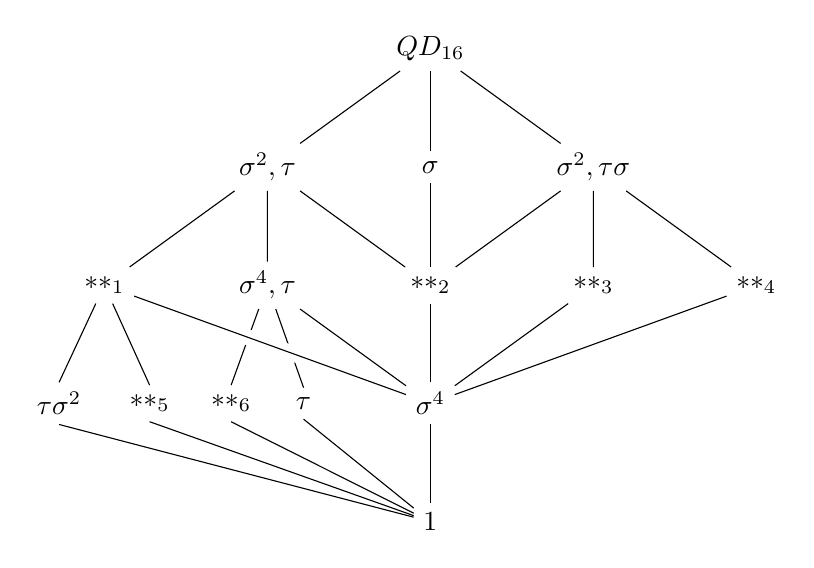
\begin{tikzpicture}[xscale=1.15, yscale=1.5]
            \node (G) at (0, 0) {$QD_{16}$};

            \node (s2t) at (-1.8, -1) {$\gen{\sigma^2, \tau}$};
            \node (s) at (0, -1) {$\gen \sigma$};
            \node (s2ts) at (1.8, -1) {$\gen{\sigma^2, \tau\sigma}$};

            \node (u1) at (-3.6, -2) {$\gen{**}_1$};
            \node (s4t) at (-1.8, -2) {$\gen{\sigma^4, \tau}$};
            \node (u2) at (0, -2) {$\gen{**}_2$};
            \node (u3) at (1.8, -2) {$\gen{**}_3$};
            \node (u4) at (3.6, -2){$\gen{**}_4$};

            \node (ts2) at (-4.1, -3) {$\gen{\tau\sigma^2}$};
            \node (u5) at (-3.1, -3) {$\gen{**}_5$};
            \node (u6) at (-2.2, -3) {$\gen{**}_6$};
            \node (t) at (-1.4, -3){$\gen \tau$};
            \node (s4) at (0, -3) {$\gen{\sigma^4}$};

            \node (1) at (0, -4) {1};

            \draw (1) -- (ts2.south);
            \draw (ts2.north) -- (u1) -- (s2t) -- (G);
            \draw (1) -- (u5.south);
            \draw (u5.north) -- (u1);
            \draw (1) -- (u6.south);
            \draw (u6.north) -- (s4t) -- (s2t);
            \draw (1) -- (t.south);
            \draw (t.north) -- (s4t);
            \draw (1) -- (s4) -- (u2) -- (s) -- (G);
            \draw [preaction={draw, line width=2mm, white}] (s4) -- (u1);
            \draw (s4) -- (s4t);
            \draw (s4) -- (u3) -- (s2ts) -- (G);
            \draw (s4) -- (u4) -- (s2ts);
            \draw (u2) -- (s2t);
            \draw (u2) -- (s2ts);
        \end{tikzpicture}
    \end{center}
    \begin{sol}
        Note that the above has been assigned subscripts to the unknown subgroups so that we may refer to them by name in the solution. To that end, note that 2 is $\gen{\sigma^2}$. To fill in the rest, we examine the cyclic subgroups for the rest of the elements. Since the structure of the subgroups generated by $\sigma^k$ are clear, we must then look to elements of the form $\tau\sigma^k$. We have
        \begin{align*}
            \gen{\tau\sigma} & = \set{1, \tau\sigma, \sigma^4, \tau\sigma^5} \\
            \gen{\tau\sigma^3} & = \set{1, \tau\sigma^3, \sigma^4, \tau\sigma^7} \\
            \gen{\tau\sigma^4} & = \set{1, \tau\sigma^4} \\
            \gen{\tau\sigma^6} & = \set{1, \tau\sigma^6}
        \end{align*}
        It becomes clear that 6 must be $\gen{\tau\sigma^4}$, since the subgroup above contains both $\tau$ and $\sigma^4$. 3 and 4 must be $\gen{\tau\sigma}$ and $\gen{\tau\sigma^3}$ respectively, since $\gen{\sigma^2, \tau\sigma}$ both contain $\tau\sigma$ and $\sigma^2$ which multiply to $\tau\sigma^3$. Certainly, 1 cannot be $\gen{\tau\sigma^6}$ as it does not contain $\gen{\tau\sigma^2}$, so it must be 5. Then 1 must be $\gen{\tau\sigma^2, \sigma^4}$ as it contains both subgroups. Hence, the completed diagram is
        \begin{center}
            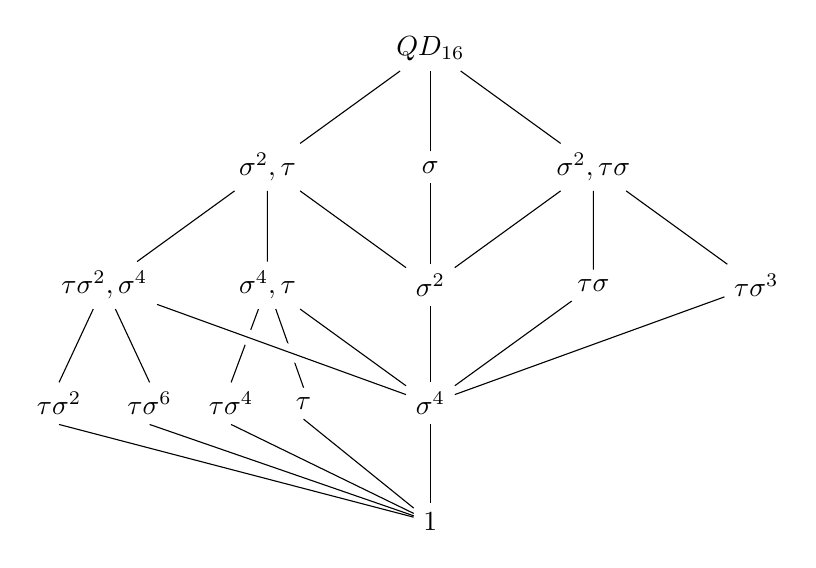
\begin{tikzpicture}[xscale=1.15, yscale=1.5]
                \node (G) at (0, 0) {$QD_{16}$};
    
                \node (s2t) at (-1.8, -1) {$\gen{\sigma^2, \tau}$};
                \node (s) at (0, -1) {$\gen \sigma$};
                \node (s2ts) at (1.8, -1) {$\gen{\sigma^2, \tau\sigma}$};
    
                \node (u1) at (-3.6, -2) {$\gen{\tau\sigma^2, \sigma^4}$};
                \node (s4t) at (-1.8, -2) {$\gen{\sigma^4, \tau}$};
                \node (u2) at (0, -2) {$\gen{\sigma^2}$};
                \node (u3) at (1.8, -2) {$\gen{\tau\sigma}$};
                \node (u4) at (3.6, -2){$\gen{\tau\sigma^3}$};
    
                \node (ts2) at (-4.1, -3) {$\gen{\tau\sigma^2}$};
                \node (u5) at (-3.1, -3) {$\gen{\tau\sigma^6}$};
                \node (u6) at (-2.2, -3) {$\gen{\tau\sigma^4}$};
                \node (t) at (-1.4, -3){$\gen \tau$};
                \node (s4) at (0, -3) {$\gen{\sigma^4}$};
    
                \node (1) at (0, -4) {1};
    
                \draw (1) -- (ts2.south);
                \draw (ts2.north) -- (u1) -- (s2t) -- (G);
                \draw (1) -- (u5.south);
                \draw (u5.north) -- (u1);
                \draw (1) -- (u6.south);
                \draw (u6.north) -- (s4t) -- (s2t);
                \draw (1) -- (t.south);
                \draw (t.north) -- (s4t);
                \draw (1) -- (s4) -- (u2) -- (s) -- (G);
                \draw [preaction={draw, line width=2mm, white}] (s4) -- (u1);
                \draw (s4) -- (s4t);
                \draw (s4) -- (u3) -- (s2ts) -- (G);
                \draw (s4) -- (u4) -- (s2ts);
                \draw (u2) -- (s2t);
                \draw (u2) -- (s2ts);
            \end{tikzpicture}
        \end{center}
    \end{sol}
\end{problems}

The next three examples lead to two nonisomorphic groups that have the same lattice of subgroups.

\begin{problems}[resume]
    \item \label{ex2.5.12} The group $A = Z_2 \times Z_4 = \gen{a, b \mid a^2 = b^4 = 1, ab = ba}$ has order 8 and has three subgroups of order 4: $\gen{a, b^2} \cong V_4, \gen b \cong Z_4$, and $\gen{ab} \cong Z_4$ and every proper subgroup is contained in one of these three. Draw the lattice of all subgroups of $A$, giving each subgroup in terms of at most two generators.
    \begin{sol}
        First, $A$ is abelian, so we may write out the elements of $A$ as
        \[A = \set{1, b, b^2, b^3, a, ab, ab^2, ab^3}\]
        Moreover, we know that $\gen{a, b^2}$ must have 3 subgroups of order 2, namely $\gen a, \gen{b^2}$, and $\gen{ab^2}$. $\gen b$ has one subgroup of order 2, $\gen{b^2}$, and $\gen{ab}$ has one subgroup of order 2, $\gen{b^2}$. We may then form the lattice:
        \begin{center}
            \begin{tikzpicture}[every node/.style=on grid]
                \node (A) {$A$};
                \node (ab) [below=of A] {$\gen{ab}$};
                \node (a b2) [below right=of A] {$\gen{a, b^2}$};
                \node (b) [below left=of A] {$\gen b$};

                \node (b2) [below right=of b] {$\gen{b^2}$};
                \node (a) [below=of a b2] {$\gen a$};
                \node (ab2) [below right=of a b2] {$\gen{ab^2}$};

                \node (1) [below= of a] {1};

                \draw (1) -- (b2) -- (ab) -- (A);
                \draw (1) -- (ab2) -- (a b2) -- (A);
                \draw (1) -- (a) -- (a b2);
                \draw (b2) -- (b) -- (A);
                \draw (b2) -- (a b2);
            \end{tikzpicture}
        \end{center}
    \end{sol}
    \item The group $G = Z_2 \times Z_8 = \gen{x, y \mid x^2 = y^8 = 1, xy = yx}$ has order 16 and has three subgroups of order 8: $\gen{x, y^2} \cong Z_2 \times Z_4, \gen y \cong Z_8$, and $\gen{xy} \cong Z_8$, and every proper subgroup is contained in one of those three. Draw the lattice of all subgroups of $G$, giving each subgroups in terms of at most two generators (cf. Exercise 12).
    \begin{sol}
        Using $a = x$ and $b = y^2$ in the previous exercise, the subgroup lattice of $G$ contains a copy of the previous lattice as well as the maximal subgroups $\gen y$ and $\gen{xy}$. We then have the lattice
        \begin{center}
            \begin{tikzpicture}[every node/.style=on grid]
                \node (G) {$G$};

                \node (y) [below left=of G] {$\gen y$};
                \node (xy) [below=of G] {$\gen{xy}$};
                \node (x y2) [below right=of G] {$\gen{x, y^2}$};

                \node (y2) [below right=of y] {$\gen{y^2}$};
                \node (xy2) [below=of x y2] {$\gen{xy^2}$};
                \node (x y4) [below right=of x y2] {$\gen{x, y^4}$};

                \node (y4) [below right=of y2] {$\gen{y^4}$};
                \node (x) [below=of x y4] {$\gen x$};
                \node (xy4) [below right= of x y4]{$\gen{xy^4}$};

                \node (1) [below=of x] {1};

                \draw (1) -- (y4) -- (y2) -- (y) -- (G);
                \draw (1) -- (xy4) -- (x y4) -- (x y2) -- (G);
                \draw (1) -- (x) -- (x y4);
                \draw (y4) -- (xy2) -- (x y2);
                \draw (y2) -- (xy) -- (G);
                \draw (y4) -- (x y4);
                \draw (y2) -- (x y2);
            \end{tikzpicture}
        \end{center}
    \end{sol}
    \item \label{ex2.5.14} Let $M$ be the group of order 16 with the following presentation:
    \[\gen{u, v \mid u^2 = v^8 = 1, vu = uv^5}\]
    (sometimes called the \textit{modular} group of order 16). It has three subgroups of order 8: $\gen{u, v^2}, \gen v$, and $\gen{uv}$, and every proper subgroup is contained in one of those three. Prove that $\gen{u, v^2} \cong Z_2 \times Z_4, \gen v \cong Z_8$, and $\gen{uv} \cong Z_8$. Show that the lattice of subgroups of $M$ is the same as the lattice of subgroups of $Z_2 \times Z_8$ (cf. Exercise 13) but that these two groups are not isomorphic.
    \begin{sol}
        Using the presentation for $Z_2 \times Z_4$ in Exercise 12, note that $u^2 = (v^2)^4 = 1$, and $v^2u = vuv^5 = uv^{10} = uv^2$, then $\gen{u, v^2}$ is an abelian subgroup of $M$, and the map $\phi : Z_2 \times Z_4 \to \gen{u, v^2}$ defined by
        \[\phi(a) = u, \quad \phi(b) = v^2\]
        is a homomorphism. Moreover, $\phi$ is surjective by construction as $\gen{u, v^2} = \gen{\phi(a), \phi(b)}$. Since $\abs{Z_2 \times Z_4} = \abs{\gen{u, v^2}}$, then $\phi$ is bijective so that $Z_2 \times Z_4 \cong \gen{u, v^2}$. Now, $\gen v$ and $\gen{uv}$ are both subgroups of order 8. Then $\gen v \cong Z_8$ and $\gen{uv} \cong Z_8$ since cyclic groups of the same order are isomorphic. Then the lattice of subgroups of $M$ is the same as the lattice of $Z_2 \times Z_8$, where $x = u$ and $y = v$:
        \begin{center}
            \begin{tikzpicture}[every node/.style=on grid]
                \node (G) {$G$};

                \node (y) [below left=of G] {$\gen v$};
                \node (xy) [below=of G] {$\gen{uv}$};
                \node (x y2) [below right=of G] {$\gen{u, v^2}$};

                \node (y2) [below right=of y] {$\gen{v^2}$};
                \node (xy2) [below=of x y2] {$\gen{uv^2}$};
                \node (x y4) [below right=of x y2] {$\gen{u, v^4}$};

                \node (y4) [below right=of y2] {$\gen{v^4}$};
                \node (x) [below=of x y4] {$\gen u$};
                \node (xy4) [below right= of x y4]{$\gen{uv^4}$};

                \node (1) [below=of x] {1};

                \draw (1) -- (y4) -- (y2) -- (y) -- (G);
                \draw (1) -- (xy4) -- (x y4) -- (x y2) -- (G);
                \draw (1) -- (x) -- (x y4);
                \draw (y4) -- (xy2) -- (x y2);
                \draw (y2) -- (xy) -- (G);
                \draw (y4) -- (x y4);
                \draw (y2) -- (x y2);
            \end{tikzpicture}
        \end{center}
        Lastly, these two subgroups are not isomorphic since $M$ is not abelian, but $Z_2 \times Z_8$ is: if it were, then $uv = vu$, but $vu = uv^5 = uv$ would imply that $v^4 = 1$, contradicting that $\abs v = 8$.
    \end{sol}
    \item Describe the isomorphism type of each of the three subgroups of $D_{16}$ of order 8.
    \begin{sol}
        Since $\abs r = 8$, then $\gen r \cong Z_8$. For the remaining subgroups, note that the lattice for $D_{16}$ shows a striking similarity to the lattice for $D_8$; in fact, these subgroups \textit{are} isomorphic to $D_8$ as follows:
        
        For the subgroup $\gen{s, r^2}$, observe that $(r^2)4 = s^2 = 1$, and $sr^2 = r^6s = (r^2)\inv s$. Then the mapping $\phi : D_8 \to \gen{s, r^2}$ given by
        \[\phi(r) = r^2, \quad \phi(s) = s\]
        extends to a homomorphism. Moreover, this mapping is surjective by construction. Since $\gen{s, r^2}$ contains a subgroup of order 4 and is a subgroup of $D_{16}$, it must be 8 so that $\phi$ is an isomorphism, and $D_8 \cong \gen{s, r^2}$.
        
        For the subgroup $\gen{sr, r^2}$, we again observe that $(r^2)^4 = (sr)^2 = 1$, and $(sr)r^2 = sr^3 = r^5s = r^6r^7s = (r^2)\inv(sr)$. The mapping $\psi : D_8 \to \gen{sr, r^2}$ given by
        \[\phi(r) = r^2, \phi(s) = sr\]
        extends to a homomorphism, surjective by construction, and is an isomorphism because $\gen{sr, r^2}$ has order 8. Then $D_8 \cong \gen{sr, r^2}$.
    \end{sol}
    \item Use the lattice of subgroups of the quasidihedral of order 16 to show that every element of order 2 is contained in the proper subgroup $\gen{\tau, \sigma^2}$ (cf. Exercise 11).
    \begin{sol}
        Every element of order 2 generates a cyclic subgroup of order 2. Using the lattice, $\gen{\tau, \sigma^2}$ properly contains all cyclic subgroups, except $\gen{\tau\sigma}$ and $\gen{\tau\sigma^3}$, both of which are order 4. Then $\gen{\tau, \sigma^2}$ contains all cyclic subgroups of order 2, hence contain all elements of order 2.
    \end{sol}
    \item Use the lattice of subgroups of the modular group $M$ of order 16 to show that the set $\set{x \in M \mid x^2 = 1}$ is a subgroup of $M$ isomorphic to the Klein 4-group (cf. Exercise 14).
    \begin{sol}
        Using the lattice in Exercise 14, we see that we have 3 candidates to be isomorphic to $V_4$, namely $\gen{v^2}, \gen{uv^2},$ and $\gen{u, v^4}$. The first and second subgroups are cyclic, while $\gen{u, v^4} = \set{1, u, v^4, uv^4}$. Since it is not generated by one element, each of these elements are of order 2, and $v^4u = v^3uv^5 = \cdots = uv^{20} = uv^4$ so that it is abelian, then $\gen{u, v^4} \cong V_4$.
    \end{sol}
    \item Use the lattice to help find the centralizer of every element of $QD_{16}$ (cf. Exercise 11).
    \begin{sol}
        Note that $\sigma^4\tau = \sigma^3\tau\sigma^3 = \cdots = \tau\sigma^{12} = \tau\sigma^4$ so that $\sigma^4 \in Z(QD_{16})$ as $\sigma^4$ already commutes with powers of $\sigma$. Moreover, any power of $\sigma$ does not commute with $\tau$ except for $\sigma^4$. The elements $\tau\sigma$ and $\tau\sigma^3$ do not commute with $\sigma^2$ as $(\tau\sigma)\sigma^2 = \tau\sigma^3 = \sigma\tau \neq \sigma^2(\tau\sigma) = \tau\sigma^2$, and $(\tau\sigma^3)\sigma^2 = \sigma^7\tau \neq \sigma^3\tau = \sigma^2(\tau\sigma^3)$. Next, $(\tau\sigma^2)\sigma^2 = \tau\sigma^4 \neq \tau = \sigma^2(\tau\sigma^2)$ so that $\sigma^2$ does not commute with $\tau\sigma^2$. Moreover, $(\tau\sigma^6)(\tau\sigma^2) = \tau\sigma^2\sigma^4\tau\sigma^2 = (\tau\sigma^2)(\tau\sigma^6)$ so that $\tau\sigma^2$ commutes with $\tau\sigma^6$, but $\sigma^2\tau\sigma^6 = \tau\sigma^4 \neq \tau = (\tau\sigma^6)\sigma^2$ so $\sigma^2$ does not commute with $\tau\sigma^6$. Lastly, $\sigma^2(\tau\sigma^4) = \tau\sigma^2 \neq (\tau\sigma^4)\sigma^2$, and $\sigma^2\tau = \tau\sigma^6 \neq \tau\sigma^2$ so that $\sigma^2$ does not commute with $\tau\sigma^4$ nor with $\tau$. It follows that the centralizers of the elements of $QD_{16}$ are
        \begin{align*}
            C_{QD_{16}}(1) = C_{QD_{16}}(\sigma^4) & = QD_{16} \\
            C_{QD_{16}}(\gen{\sigma^k}) & = \gen\sigma \text{ for $k = 1, 2, 3, 5, 6, 7$} \\
            C_{QD_{16}}(\gen{\tau\sigma}) = C_{QD_{16}}(\gen{\tau\sigma^5}) & = \gen{\tau\sigma} \\
            C_{QD_{16}}(\gen{\tau\sigma^3}) = C_{QD_{16}}(\gen{\tau\sigma^7}) & = \gen{\tau\sigma^3} \\
            C_{QD_{16}}(\gen\tau) = C_{QD_{16}}(\gen{\tau\sigma^4}) & = \gen{\sigma^4, \tau} \\
            C_{QD_{16}}(\gen{\tau\sigma^2}) = C_{QD_{16}}(\gen{\tau\sigma^6}) & = \gen{\tau\sigma^2, \sigma^4}
        \end{align*}
    \end{sol}
    \item Use the lattice to help find $N_{D_{16}}(\gen{s, r^4})$.
    \begin{sol}
        Based on the placement of $\gen{s, r^4}$, its normalizer may be itself, $\gen{s, r^2}$, or $D_{16}$. Note that $\gen{s, r^4} = \{1, s, r^4, sr^4\}$, and taking $r^2$ and $(r^2)\inv = r^6$, we have
        \[r^2\gen{s, r^4}r^6 = \set{1, sr^4, r^4, s} = \gen{s, r^4}\]
        so that $r^2 \in N_{D_{16}}(\gen{s, r^4})$, and $\gen{s, r^2} \leq N_{D_{16}}(\gen{s, r^4})$. Since $rsr\inv = r^2s \neq r$, then $r \not\in N_{D_{16}}(\gen{s, r^4})$ so that $N_{D_{16}}(\gen{s, r^4}) = \gen{s, r^2}$.
    \end{sol}
    \item Use the lattice of subgroups of $QD_{16}$ (cf. Exercise 11) to help find the normalizers
    \begin{problems}
        \item $N_{QD_{16}}(\gen{\tau\sigma})$
        \item $N_{QD_{16}}(\gen{\tau, \sigma^4})$.
    \end{problems}
    \begin{solalph}
        \item Note that $\gen{\tau\sigma} = \set{1, \tau\sigma, \sigma^4, \tau\sigma^5}$. Moreover, $(\sigma^2)\inv = \sigma^6$ so that
        \[\sigma^2\gen{\tau\sigma}\sigma^6 = \{1, \tau\sigma^4, \sigma^4, \tau\sigma\} = \gen{\tau\sigma}\]
        and $\sigma(\tau\sigma)\sigma^7 = \tau\sigma^3 \neq \tau\sigma$ so that $\sigma \not\in N_{QD_{16}}(\gen{\tau\sigma})$ so that $N_{QD_{16}}(\gen{\tau\sigma}) = \gen{\sigma^2, \tau\sigma}$.
        \item $\gen{\tau, \sigma^4} = \{1, \tau, \sigma^4, \tau\sigma^4\}$, and 
        \[z\sigma^2\gen{\tau, \sigma^4}\sigma^6 = \{1, \tau\sigma^4, \sigma^4, \tau\}\]
        while $\sigma\tau\sigma^7 = \tau\sigma^2 \neq \tau$ so that $\sigma \not\in N_{QD_{16}}(\gen{\tau, \sigma^4})$. Then $N_{QD_{16}}(\gen{\tau, \sigma^4}) = \gen{\sigma^2, \tau}$.
    \end{solalph}
\end{problems}